% ============================================================
% CEAZA Coastal Sensor Reconstruction --- Internship Report
% Case Study 1: Chlorophyll-a (BTGCLF channel).  Case Study 2: Dissolved Oxygen (BTGOXD2 channel).
% ============================================================
\documentclass[11pt, a4paper]{article}
\setlength{\parindent}{0pt}

% ── Packages ──────────────────────────────────────────────
\usepackage[utf8]{inputenc}
\usepackage[T1]{fontenc}
\usepackage{lmodern}
\usepackage[margin=2cm]{geometry}
\usepackage{graphicx}
\usepackage{booktabs}
\usepackage{enumitem}
\usepackage{array}
\usepackage{tabularx}
\usepackage{longtable}
\usepackage{amsmath}
\usepackage{amssymb}
\usepackage{siunitx}
\usepackage{xcolor}
\usepackage[colorlinks=true, linkcolor=black, citecolor=black, urlcolor=black,
            breaklinks=true]{hyperref}
\usepackage{natbib}
\usepackage{csvsimple}
\usepackage{tikz}
\usetikzlibrary{arrows.meta,positioning,decorations.pathreplacing}
\usepackage{placeins}
\usepackage{caption}
\usepackage{comment}
\usepackage{ragged2e}
\newcolumntype{Y}{>{\RaggedRight\arraybackslash}X}
\newcolumntype{P}[1]{>{\RaggedRight\arraybackslash}p{#1}}
\newlist{tabitemize}{itemize}{1}
\setlist[tabitemize]{
  label=\textbullet,
  leftmargin=*,
  nosep,
  topsep=0pt,
  partopsep=0pt,
  parsep=0pt,
  itemsep=0pt,
  before=\vspace{-0.6\baselineskip},
}
\usepackage{float}

% ── Float-page vertical placement ───────────────────────────
% article.cls default float-page glue (\@fptop = 0pt plus 1fil, matched by \@fpbot)
% vertically centers a lone float on a float-only page, which looks like an
% unprofessional blank gap above the figure. Zeroing \@fptop makes lone floats on
% float-only pages sit at the top of the page instead; all remaining slack goes
% below via the unchanged \@fpbot.
\makeatletter
\setlength{\@fptop}{0pt}
\makeatother

% ── Draft-status / metadata placeholder commands ────────────
\newcommand{\TODO}[1]{\textcolor{gray!70!black}{\textit{[pending: #1]}}}
\newcommand{\DRAFTMETA}[1]{\textcolor{gray!70!black}{\textit{#1}}}
\newcommand{\NOTE}[1]{\textcolor{gray}{\small\textit{Note: #1}}}

% ── Figure-slot placeholder (for figures not yet built at manuscript quality) ──
% Compact placeholder for a figure not yet built at manuscript quality: renders
% only a slim bordered box with the caption, so the compiled report reads as a
% manuscript with figures pending rather than an internal planning document. The
% full intended-message/panel/evidence-tier brief for each slot lives in a LaTeX
% comment immediately above the \FIGSLOT call in the source, and is consolidated
% in docs/project_state/FINAL_REPORT_FIGURE_STORYBOARD_D9.md for whoever builds
% the final figure. First argument is the figure label; second is the caption.
\newcommand{\FIGSLOT}[2]{%
  \begin{figure}[htbp]
    \centering
    \fbox{\begin{minipage}{0.75\textwidth}
      \centering
      \vspace{0.15cm}
      \small\textit{Figure pending --- see accompanying repository for the figure storyboard.}
      \vspace{0.15cm}
    \end{minipage}}
    \caption{#2}
    \label{fig:#1}
  \end{figure}
}

% ── Scientific shorthand ────────────────────────────────────
\newcommand{\chl}{Chl\,\textit{a}}
\DeclareSIUnit{\ug}{\micro\gram}

% ── Title ─────────────────────────────────────────────────
\title{
  Benchmarking Imputation in Sparse Coastal Sensor Records:\\
  Chlorophyll-\textit{a} and Dissolved Oxygen in Tongoy Bay, Chile
}

\author{
  Matteo Faverio
}
\date{}
% ═══════════════════════════════════════════════════════════
\begin{document}
\maketitle

% ── Abstract ──────────────────────────────────────────────
\begin{abstract}
  Coastal monitoring stations produce long in-situ time series that are chronically interrupted by
  sensor outages, often precisely when the underlying signal is most dynamic. This report develops
  and benchmarks a workflow for reconstructing these historical gaps at Tongoy Bay, Chile, using
  in-situ chlorophyll-\textit{a} (\chl{}) as the primary case study and in-situ dissolved oxygen as a second case testing whether the workflow transfers to a
  different sensor. Methods are ranked under an artificial-gap benchmark that hides observed values
  and scores each reconstruction against the withheld truth; outputs for the stations' real gaps
  have no withheld truth and are reported only as illustrative reconstructions, while being useful material for the hosting research center (CEAZA) and its modelling activities. For chlorophyll, an
  engineered tabular model built on external satellite and physical predictors never beats simple
  linear interpolation, while a pretrained time-series foundation model (TS-ICL) applied zero-shot
  is the strongest single method. An architecture-independent covariate probe finds that wind/upwelling forcing
  carries a genuine physical signal, and high-\chl{} events remain difficult for every method tested. The same model ladder transfers to oxygen: linear
  interpolation is again the floor, no engineered tabular model beats it, and TS-ICL again improves
  on the pooled average, but is weaker than interpolation in both tails of the oxygen distribution and worst in sustained
  tail episodes. Together the two cases show when model complexity helps over a strong classical floor, which physical channels carry a reconstructable signal, and where distributional extremes
  remain difficult.
\end{abstract}

% ── Sections ───────────────────────────────────────────────

% ── Section 1: Introduction ───────────────────────────────
\section{Introduction}
\label{sec:introduction}

Coastal ocean monitoring stations produce long and biologically informative time series, but they
are rarely complete: sensor outages, maintenance windows, and storm damage interrupt
the record, often precisely when the underlying signal is most dynamic and most scientifically
interesting. Reconstructing these historical gaps matters both for day-to-day monitoring and for
any downstream scientific interpretation of the record. What operational networks need is not a
one-off fix for a single station or variable, but a workflow that can be reapplied each time a
new sensor or a new gap appears \citep{moritz2017imputets}.

This report develops such a workflow for the Centro de Estudios Avanzados en Zonas \'{A}ridas
(CEAZA) network \citep{ceazamet_network} at Tongoy Bay, Chile
($\sim$30.3\textdegree{}S, 71.6\textdegree{}W; Figure~\ref{fig:site-context}), a Humboldt Current
upwelling site \citep{montecino2009humboldt} that hosts a scallop (\textit{Argopecten
purpuratus}) aquaculture industry whose production is closely tied to local phytoplankton
dynamics and to upwelling-driven variability in oxygen, temperature, and pH
\citep{ramajo2019scallops}. Two sensors on the Tongoy buoy (BTG) anchor the study: an in-situ
chlorophyll-\textit{a} (\chl{}) fluorometer, the primary case study, and a dissolved-oxygen
sensor, a second case study that tests how well the workflow transfers to a physically distinct
variable. Both records span 2015--2026 and share the buoy's missingness structure, including a
common 256-day station-wide outage during the 2020 pandemic; chlorophyll's daily record is 24.5\% missing and oxygen's is
27.8\% missing (Section~\ref{sec:data}).

Reconstructing a nearshore biological signal like \chl{} is harder than a generic gap-filling
problem, and the report treats the reasons as questions to answer:
\begin{itemize}
    \item \textbf{How strong are the simple baselines?} Linear interpolation and climatology are the floor every method must clear.
    
    \item \textbf{Do external satellite and physical products help?} Regional ocean-colour and reanalysis fields (wind, current, sea surface temperature) are continuously available during a gap, but their resolution may be too coarse for a nearshore signal.

    \item \textbf{Can a zero-shot foundation model provide an alternative?} Such models require no station-specific training and no feature engineering, which is attractive operationally.

    \item \textbf{Where do the methods fail?} The regimes of greatest interest --- short chlorophyll blooms and the tails of the oxygen distribution --- are where imputation is hardest.
\end{itemize}
 
One principle organises all of the evidence. Methods are ranked only on artificial gaps: observed values are hidden, each method reconstructs them, and the reconstruction is
scored against the withheld truth. The stations' real gaps have no ground truth, so any
reconstruction of them can be inspected for plausibility and is useful for the research center activities, but never used to rank methods. \\
The report makes two contributions.

First, it benchmarks five comparator groups for daily in-situ Chl a under an artificial-gap protocol: simple temporal baselines, a target-only Gaussian-process
smoother, an engineered tabular model using only external predictors, a gap-edge residual model
conditioned on the observations bounding each gap, and a pretrained time-series foundation model
(TS-ICL) applied zero-shot, reporting which method wins, where, and why.
Second, it carries the same target-definition, gap-audit, and model-ladder workflow through to a
second sensor, dissolved oxygen (Section~\ref{sec:oxygen}), so that the benchmark itself, and not
just the chlorophyll result, is the reusable product CEAZA can reapply to further sensors and
stations.

Section~\ref{sec:data} describes both case studies' data and target construction;
Section~\ref{sec:methodology} defines the shared benchmark;
Section~\ref{sec:chl_results} presents the chlorophyll results in full;
Section~\ref{sec:oxygen} presents the more compact oxygen case;
Section~\ref{sec:synthesis} compares what transfers between the two; and
Section~\ref{sec:limitations_future} closes with limitations and research directions.
Appendix~\ref{sec:appendix_repro} gives the compact reproducibility details and backing tables,
while the accompanying code repository contains the complete implementation and raw outputs.

\begin{figure}[h]
  \centering
  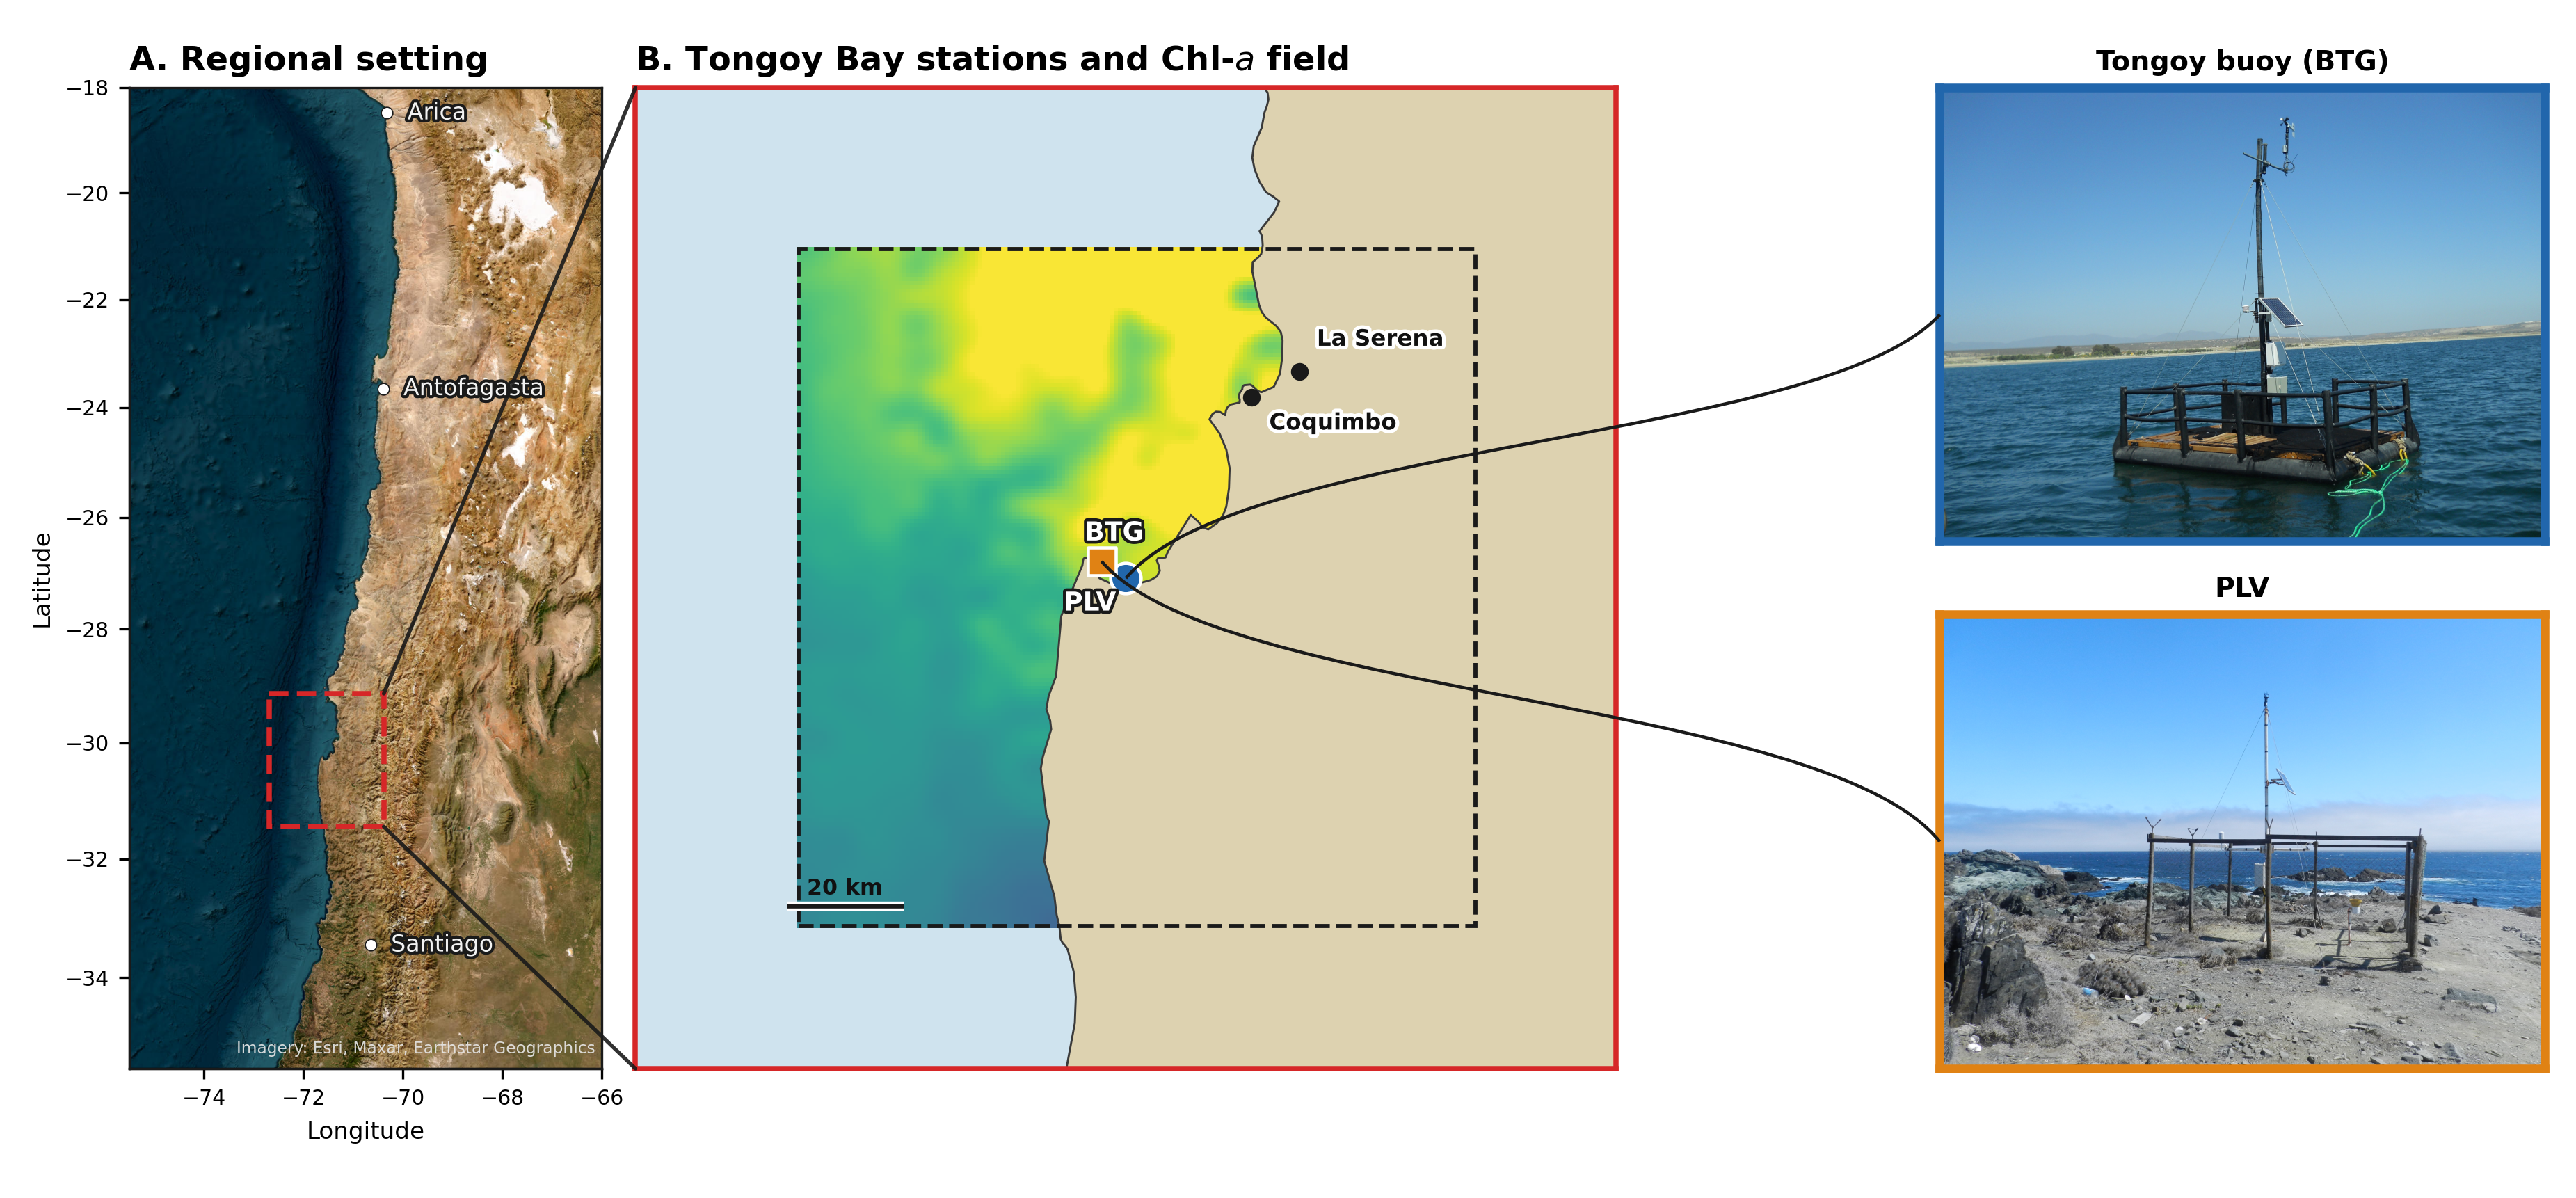
\includegraphics[width=\textwidth]{figures/fig1_site_context.png}
  \caption{Study site and monitoring context. (A) Regional setting on the north-central
  Chilean coast; (B) Tongoy Bay:
  the Tongoy buoy (BTG, carrying the chlorophyll and dissolved-oxygen sensors), the PLV
  meteorological station, the satellite/reanalysis extraction domain (dashed box), and a
  representative satellite Chl-\textit{a} field (2021-01-17), with field photographs of both installations.}
  \label{fig:site-context}
\end{figure}
\newpage
% ── Section 2: Data and case-study setting ────────────────
\section{Data and Case-Study Setting}
\label{sec:data}

\subsection{Study site and monitoring stations}

Tongoy Bay is monitored by two CEAZAMET stations \citep{ceazamet_network,ceazamet_btg_station}
(Figure~\ref{fig:site-context}): the Tongoy buoy
(BTG), a floating platform (lat~$-30.275$\textdegree{}, lon~$-71.562$\textdegree{})
carrying the in-situ chlorophyll (channel BTGCLF) and dissolved-oxygen (channel BTGOXD2) sensors
used in this report, and PLV, a coastal meteorological mast at Punta Lengua de Vaca
($\sim$15~km away), sited at a known regional
upwelling centre \citep{moraga2001plv} and providing wind, solar radiation, humidity, and
pressure. Both provide hourly observations from 2015 to 2026. Satellite and reanalysis products (chlorophyll, sea-surface temperature, wind stress, and
ocean currents) are extracted over a fixed regional box around the Tongoy coordinate and
used as external predictors in both case studies (Table~\ref{tab:data_sources}; full
extraction detail in Appendix~\ref{sec:appendix_repro}).

\begin{table}[htbp]
\centering
\caption{Main external predictor products. Product-level provenance and citations are given in
Appendix~\ref{app:data_products}.}
\label{tab:data_sources}
\small
\begin{tabular}{p{4cm}p{6cm}p{1.6cm}p{2.5cm}}
\toprule
Product & Scientific role & Coverage & Resolution \\
\midrule
GlobColour L4 \chl{} & Regional surface-biology proxy & 90\% & $\sim$4~km, daily \\
MUR SST & Thermal tracer / surface state & 98\% & $\sim$1~km, daily \\
CMEMS winds & Regional wind forcing for upwelling & 90\% & $\sim$25~km, hourly \\
PLV station & Local atmospheric forcing & 76\% & point, hourly \\
GLORYS12 currents & Shelf transport / advection predictors & $>$99\% & $\sim$8~km, daily \\
\bottomrule
\end{tabular}
\end{table}

Table~\ref{tab:data_sources} is easier to interpret in the physical setting of the Tongoy coast.
This part of northern-central Chile belongs to the Humboldt upwelling system, where
equatorward alongshore winds can drive offshore Ekman transport in the surface layer.
The resulting nearshore divergence is compensated by the upward movement of colder,
nutrient-rich subsurface water onto the shelf and into the coastal zone
\citep{kampf2016upwelling, montecino2009humboldt}. Figure~\ref{fig:upwelling_schematic}
shows this process schematically for the Tongoy Bay setting.

\begin{figure}[htbp]
  \centering
  
\includegraphics[width=0.75\textwidth]{figures/fig_upwelling_schematic.png}
  \caption{Conceptual schematic of the upwelling setting relevant to Tongoy Bay.}
  \label{fig:upwelling_schematic}
\end{figure}

This process motivates the external predictors used later in the benchmark.
Wind from PLV and reanalysis represents the mechanical forcing of upwelling,
sea-surface temperature (SST) acts as a thermal tracer of recently upwelled water and
surface stratification, satellite chlorophyll provides a biological proxy, and
ocean-current fields represent advection, exchange, and retention on the shelf.

The same predictor families are plausible for both case
studies, as their interaction can explain part of the physical process, but their usefulness will be established empirically in the benchmark.

\subsection{Case Study 1: chlorophyll-\textit{a} target, distribution, and missingness}
\label{sec:chl_target}

\noindent
\begin{minipage}[t]{0.57\textwidth}
The chlorophyll reconstruction target is the daily mean in-situ \chl{} from the Tongoy buoy
(BTG) fluorometer channel BTGCLF, expressed in mg~m\textsuperscript{$-3$} and computed from
hourly observations. A day is eligible only if at least 18 hourly values are valid
(coverage $\geq 75\%$); otherwise it is excluded from the target and treated as missing.
The eligible daily distribution is strongly right-skewed, with intermittent
high-concentration days (Figure~\ref{fig:chl_distribution}). For this reason, all models
are fitted on $\log_{10}(\texttt{chl\_mean})$, while physical-unit values are retained for
interpretation.

\medskip

Over 3988 days (2015-07-01 to 2026-05-31), 3012 (75.5\%) are eligible and 976
are missing, forming 128 real gaps (Figure~\ref{fig:chl_target_and_gaps}). Most gaps are
brief interruptions, but the record also contains a 256-day gap from 2020-02-11 to
2020-10-23. This very long gap spans three seasons and
is treated only as an illustrative reconstruction scenario because no validation is available for such long gaps.
\end{minipage}
\hfill
\begin{minipage}[t]{0.39\textwidth}
\vspace{-0.6em}
\centering
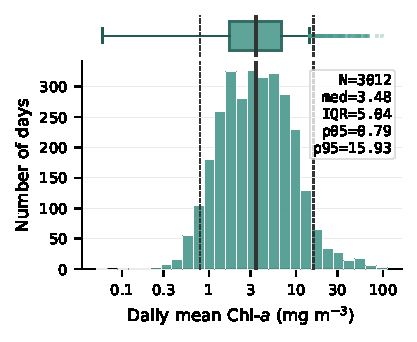
\includegraphics[width=\linewidth]{figures/fig_chl_distribution.pdf}
\captionsetup{justification=raggedright,singlelinecheck=false,font=footnotesize}
\captionof{figure}{Distribution of eligible daily chlorophyll-\textit{a}. The solid line marks
the median; dashed lines mark p05 and p95.}
\label{fig:chl_distribution}
\end{minipage}

\vspace{0.8em}

\begin{figure}[htbp]
  \centering
  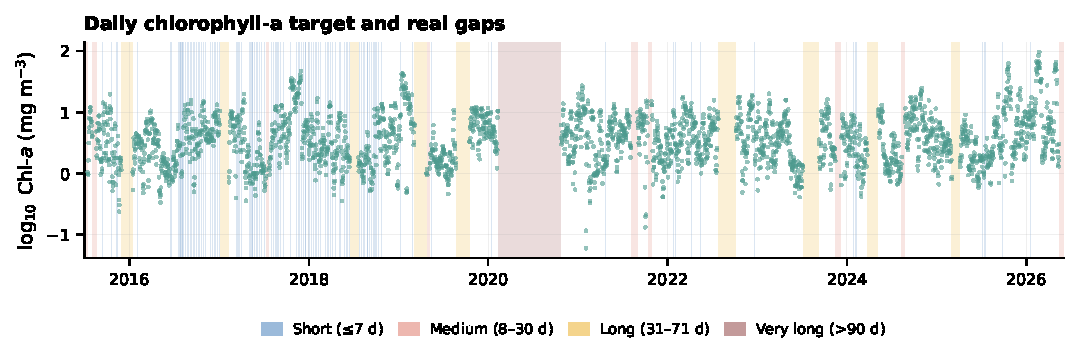
\includegraphics[width=0.96\textwidth]{figures/fig_chl_target_and_gaps.pdf}
  \caption{Observed daily chlorophyll-\textit{a} and real-gap structure at Tongoy buoy (BTG).}
  \label{fig:chl_target_and_gaps}
\end{figure}

\subsection{Case Study 2: dissolved oxygen target, distribution, and missingness}
\label{sec:oxygen_data}

\noindent
\begin{minipage}[t]{0.57\textwidth}
The dissolved oxygen reconstruction target is the daily mean oxygen concentration from the
Tongoy buoy (BTG) sensor channel BTGOXD2, expressed in mg/L and computed from hourly
observations. The same daily eligibility rule is used as for chlorophyll: a day enters the
target only if at least 18 hourly values are valid. Across eligible days, the distribution
has median 6.429~mg/L, with p05 2.818~mg/L and p95 8.802~mg/L, and includes both low and
high tails (Figure~\ref{fig:oxygen_distribution}).

\medskip

Over the same 3988-day span (2015-07-01 to 2026-05-31), 2880 days (72.2\%) are eligible
and 1108 are missing or ineligible, forming 125 real gaps
(Figure~\ref{fig:oxygen_target_and_gaps}). The three largest are a 256-day gap shared with
chlorophyll from 2020-02-11 to 2020-10-23, a 161-day oxygen-specific gap from 2025-02-08
to 2025-07-18, and a 71-day gap from 2022-07-27 to 2022-10-05. 
\end{minipage}
\hfill
\begin{minipage}[t]{0.39\textwidth}
\vspace{-0.6em}
\centering
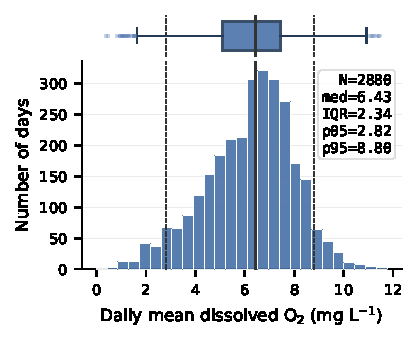
\includegraphics[width=\linewidth]{figures/fig_oxygen_distribution.pdf}
\captionsetup{justification=raggedright,singlelinecheck=false,font=footnotesize}
\captionof{figure}{Distribution of eligible daily dissolved oxygen. The solid line marks
the median; dashed lines mark p05 and p95.}
\label{fig:oxygen_distribution}
\end{minipage}

\vspace{0.8em}

\begin{figure}[htbp]
  \centering
  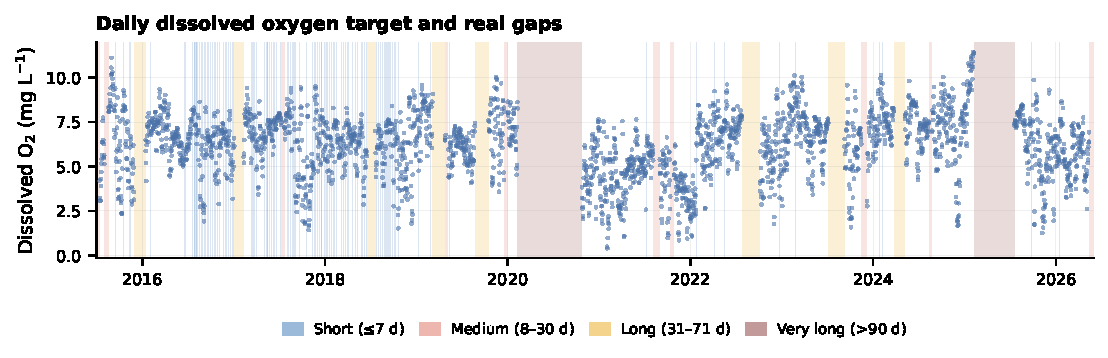
\includegraphics[width=0.96\textwidth]{figures/fig_oxygen_target_and_gaps.pdf}
  \caption{Observed daily dissolved oxygen and real-gap structure at Tongoy buoy (BTG).}
  \label{fig:oxygen_target_and_gaps}
\end{figure}

\subsection{Predictor channels and feature construction}
\label{sec:predictors}

The data products introduced above are converted into predictor channels before modelling.
These channels summarize five types of information: seasonality, target history outside the
hidden gap, satellite biological signal, atmospheric/upwelling forcing, and ocean
current/transport conditions (Table~\ref{tab:predictor_families}). Feature construction is both
temporal and spatial. Temporal features include lags, rolling means, cumulative indices, and
pre-/post-gap boundary summaries. Spatial features summarize gridded products around Tongoy, for example through nearest-cell values, regional means, local variability, or
coastal gradients. This avoids reducing every external product to a single nearest pixel.

\begin{table}[htbp]
\centering
\caption{Predictor channels and representative feature constructions. Full feature lists are
given in Appendix~\ref{sec:appendix_repro}.}
\label{tab:predictor_families}
\small
\renewcommand{\arraystretch}{1.15}
\begin{tabularx}{\textwidth}{P{3.0cm}Y Y}
\toprule
Channel & What is encoded & Representative features \\
\midrule
Calendar / seasonality
& Position within the annual cycle.
& Month; $\sin$/$\cos$ day-of-year terms. \\

Target history / gap-edge context
& Observed target behaviour immediately outside the hidden gap.
& Last pre-gap value; 7-d pre-gap mean and slope; first post-gap value; post-gap mean;
edge-to-edge change and slope. \\

Satellite biological proxy
& Regional surface chlorophyll information from satellite products.
& Nearby or regional $\log_{10}$ \chl{}; local box means; chlorophyll anomaly; valid-pixel
fraction; patchiness metrics. \\

Atmospheric / upwelling forcing
& Wind, radiation, SST, and upwelling-related surface forcing.
& PLV solar radiation; wind speed; cumulative upwelling index; rolling SST; recent SST
cooling. \\

Ocean current / transport
& Advection, exchange, and retention conditions over the regional extraction box.
& Surface current speed; alongshore current component;
Okubo--Weiss-type transport summaries. \\
\bottomrule
\end{tabularx}
\end{table}

The representation of these channels depends on the model family. Tabular models see one
feature vector per target day, so temporal and spatial context must be encoded explicitly in
the columns. This is why the tabular feature set contains rolling windows, lags, cumulative
forcing indices, regional summaries, and gap-edge statistics. TS-ICL instead receives
time-indexed target and covariate sequences over a context window. Its covariates can still be
engineered channels, but they are supplied as sequences rather than collapsed into a single
row. Therefore, the same scientific information families can be used across model families
without requiring the exact same feature representation.
\newpage
% ── Section 3: Benchmark methodology ──────────────────────
\section{Benchmark Methodology}
\label{sec:methodology}

This section defines the benchmark used to compare reconstruction methods for the two sensor
targets. The benchmark asks how well different information sources can recover missing values in
a historical daily record: local target continuity, external physical covariates, gap-edge
context, and pretrained sequence modelling. Internal gaps are treated as historical imputation
problems, so observations on both sides of the missing interval may be used when available.

\subsection{Model ladder}
\label{sec:model_ladder}

Let $y_t$ denote the daily target on its modelling scale, and let
$\mathbf{x}_t$ denote the external covariate information available at day $t$. For an artificial
gap
\[
    G=\{t_0,\ldots,t_0+L-1\},
\]
the values $\mathbf y_G=\{y_t:t\in G\}$ are hidden and reconstructed as
$\hat{\mathbf y}_G=\{\hat y_t:t\in G\}$. All methods solve this same reconstruction problem, but
they differ in the information representation they use: simple temporal rules, target-only
continuity, external covariate features, explicit gap-edge context, or a pretrained sequence
model.

\begin{figure}[htbp]
  \centering
  \makebox[\textwidth][c]{%
    \hspace*{-1.5cm}%
    \resizebox{1.01\textwidth}{!}{% TikZ source: model-ladder hero figure with embedded generated subfigures.
% Included via:
%   \resizebox{\textwidth}{!}{% TikZ source: model-ladder hero figure with embedded generated subfigures.
% Included via:
%   \resizebox{\textwidth}{!}{\input{figures/fig_model_ladder_tikz.tex}}
%
% Requires graphicx in preamble.
% Expected external files (optional; fallback box shown if absent):
%   figures/model_ladder_external_tabular.png
%   figures/model_ladder_gap_edge_residual.png
%   figures/model_ladder_tsicl.png

\definecolor{vgTarget}{HTML}{2A7F8E}  % observed target (teal)
\definecolor{vgRecon}{HTML}{1B9E77}   % reconstruction / smoother output (green)
\definecolor{vgExt}{HTML}{3B6FA0}     % external predictors / features (blue)
\definecolor{vgEdge}{HTML}{D98A2B}    % gap-edge / residual correction (amber)
\definecolor{vgPrior}{HTML}{7E6CA8}   % TS-ICL / pretrained sequence model (violet)
\definecolor{vgHidden}{HTML}{C0504D}  % hidden gap (red)
\definecolor{vgInk}{HTML}{2B2B2B}     % text
\definecolor{vgFaint}{HTML}{9AA6B2}   % row tags / faint rules
\definecolor{vgGrid}{HTML}{D9DEE2}    % daily time grid
\definecolor{vgArrow}{HTML}{8A9299}   % flow arrows
\definecolor{vgPanel}{HTML}{F7F8F9}   % panel background
\definecolor{vgChip}{HTML}{ECEFF2}    % model chip fill

\definecolor{mBase}{HTML}{5F7F8A}     % simple baselines
\definecolor{mGP}{HTML}{1B9E77}       % Gaussian process
\definecolor{mExt}{HTML}{3B6FA0}      % external tabular
\definecolor{mGap}{HTML}{D98A2B}      % gap-edge residual
\definecolor{mTS}{HTML}{7E6CA8}       % TS-ICL
\definecolor{tsgreen}{HTML}{08A69B}
\definecolor{tsblue}{HTML}{004CF8}


\begin{tikzpicture}[x=0.38cm, y=0.38cm, font=\small,
    flow/.style={-{Latex[length=2mm]}, vgArrow, line width=0.9pt}]

  % ---------------------------------------------------------------------------
  % Global geometry
  % ---------------------------------------------------------------------------
  \def\PW{9.7}        % panel width
  \def\PH{24.9}       % panel height
  \def\DX{10.55}      % horizontal shift between panels

  \def\Ytitle{23.95}
  \def\YmodelA{20.60}
  \def\YmodelB{22.70}
  \def\YhowA{10.45}
  \def\YhowB{19.75}
  \def\YoutA{1.55}
  \def\YoutB{9.20}

  \def\Yeq{7.65}      % equation height inside output box
  \def\ob{2.95}       % baseline of output mini-plots

  % ---------------------------------------------------------------------------
  % Helpers
  % ---------------------------------------------------------------------------

  \newcommand{\panelbg}[2]{%
    \fill[vgPanel, rounded corners=3pt] (-0.25,0.75) rectangle (\PW,\PH);
    \draw[#2, opacity=0.45, line width=0.65pt, rounded corners=3pt]
      (-0.25,0.75) rectangle (\PW,\PH);
    \node[font=\small\bfseries, text=vgInk, align=center] at (4.72,\Ytitle) {#1};
  }

  \newcommand{\modelchip}[1]{%
    \fill[vgChip, rounded corners=3pt] (1.05,\YmodelA) rectangle (8.40,\YmodelB);
    \draw[#1, opacity=0.40, line width=0.55pt, rounded corners=3pt]
      (1.05,\YmodelA) rectangle (8.40,\YmodelB);
  }

  \newcommand{\howbox}[1]{%
    \fill[#1, opacity=0.040, rounded corners=3pt] (0.55,\YhowA) rectangle (8.95,\YhowB);
    \draw[#1, opacity=0.75, line width=0.7pt, rounded corners=3pt]
      (0.55,\YhowA) rectangle (8.95,\YhowB);
  }

  \newcommand{\outbox}[1]{%
    \fill[#1, opacity=0.040, rounded corners=3pt] (0.55,\YoutA) rectangle (8.95,\YoutB);
    \draw[#1, opacity=0.75, line width=0.7pt, rounded corners=3pt]
      (0.55,\YoutA) rectangle (8.95,\YoutB);
  }

  \newcommand{\imageorfallback}[3]{%
    \IfFileExists{#1}{%
      \includegraphics[width=#2]{#1}%
    }{%
      \fbox{\parbox[c][2.8cm][c]{#2}{\centering\scriptsize #3}}%
    }%
  }

  % output grid with observed context and hidden interval
  \newcommand{\miniout}[1]{%
    \foreach \s in {1,...,9}{
      \draw[vgGrid,line width=0.28pt](0.2+\s*0.9,#1)--(0.2+\s*0.9,#1+3.3);
    }
    \fill[vgHidden,opacity=0.12](0.2+3.5*0.9,#1)rectangle(0.2+6.5*0.9,#1+3.3);
    \draw[vgTarget,line width=1.0pt](1.1,#1+1.35)--(2.0,#1+1.00)--(2.9,#1+1.20);
    \draw[vgTarget,line width=1.0pt](6.5,#1+2.50)--(7.4,#1+2.85)--(8.3,#1+2.50);
    \foreach \s/\y in {1/1.35,2/1.00,3/1.20,7/2.50,8/2.85,9/2.50}{
      \fill[vgTarget](0.2+\s*0.9,#1+\y)circle(0.10);
    }
  }

  % compact target-gap sketch used in "how" boxes
  \newcommand{\howgap}[1]{%
    \foreach \s in {1,...,9}{
      \draw[vgGrid,line width=0.25pt](0.2+\s*0.9,#1)--(0.2+\s*0.9,#1+3.3);
    }
    \fill[vgHidden,opacity=0.12](0.2+3.5*0.9,#1)rectangle(0.2+6.5*0.9,#1+3.3);
    \draw[vgTarget,line width=0.95pt](1.1,#1+1.35)--(2.0,#1+1.00)--(2.9,#1+1.20);
    \draw[vgTarget,line width=0.95pt](6.5,#1+2.50)--(7.4,#1+2.85)--(8.3,#1+2.50);
    \foreach \s/\y in {1/1.35,2/1.00,3/1.20,7/2.50,8/2.85,9/2.50}{
      \fill[vgTarget](0.2+\s*0.9,#1+\y)circle(0.09);
    }
  }

  % left row labels
  \node[rotate=90,font=\footnotesize\bfseries,text=vgFaint] at (-2.25,22.10) {METHOD};
  \node[rotate=90,font=\footnotesize\bfseries,text=vgFaint] at (-2.25,15.10) {MECHANISM};
  \node[rotate=90,font=\footnotesize\bfseries,text=vgFaint] at (-2.25,5.35) {OUTPUT};

  % ---------------------------------------------------------------------------
  % Panel 1: Simple baselines
  % ---------------------------------------------------------------------------
  \begin{scope}[shift={(0,0)}]
    \panelbg{Simple baselines}{mBase}
    \modelchip{mBase}
    \node[font=\tiny, text=vgInk, align=center, text width=3.2cm] at (4.72,21.65)
      {climatology\\persistence\\linear interpolation};

    \howbox{mBase}
    % three rule sketches with equations, not names
    \def\yshift{-0.9}
\foreach \yy/\eqn in {
  17.90/{{$\hat y_t = y_{t^-}$}},
  15.90/{{$\hat y_t=\tilde y_t^{\mathrm{lin}}$}},
  13.90/{{$\hat y_t = \mu_{\mathrm{season}}$}}
}{
  \fill[vgHidden,opacity=0.12](1.35,\yy-0.55+\yshift) rectangle (2.30,\yy+0.55+\yshift);
  \fill[vgTarget](0.95,\yy-0.25+\yshift) circle(0.09);
  \fill[vgTarget](2.80,\yy+0.30+\yshift) circle(0.09);
  \node[font=\scriptsize,text=vgInk,anchor=west] at (3.60,\yy+\yshift) {\eqn};
}
    % persistence
    \draw[mBase,line width=1.35pt] (0.95,16.75)--(2.80,16.75);
    % interpolation
    \draw[mBase,line width=1.35pt] (0.95,14.75)--(2.80,15.30);
    % climatology
    \draw[mBase,line width=1.35pt] (0.95,13)--(2.80,13);

    \draw[flow] (4.75,20.35)--(4.75,19.95);
    \draw[flow] (4.75,10.25)--(4.75,9.55);

    \outbox{mBase}
    \node[font=\scriptsize,text=vgInk,align=center] at (4.75,\Yeq)
      {$\hat y_t=\tilde y_t^{\mathrm{lin}}$};
    \miniout{\ob}
    % only interpolation shown in output
    \draw[mBase,line width=1.6pt](2.9,\ob+1.2)--(6.5,\ob+2.5);
    \foreach \s in {4,5,6}{
      \fill[mBase](0.2+\s*0.9,{\ob+1.2+(\s-3)*0.325})circle(0.10);
    }
  \end{scope}

  % ---------------------------------------------------------------------------
  % Panel 2: Target-only smoother
  % ---------------------------------------------------------------------------
  \begin{scope}[shift={(\DX,0)}]
    \panelbg{\scalebox{0.93}{Target-only smoother}}{mGP}
    \modelchip{mGP}
    \node[font=\scriptsize, text=vgInk, align=center, text width=3.0cm] at (4.72,21.65)
      {Gaussian process};

    \howbox{mGP}

\begin{scope}[yshift=-0.35cm]
\howgap{13.85}

% Prior mean m(t): faint dashed reference trend
\draw[vgFaint,line width=0.75pt,dash pattern=on 2pt off 1.5pt]
  plot[smooth] coordinates{
    (1.1,15.20)
    (2.9,15.10)
    (4.7,15.70)
    (6.5,16.35)
    (8.3,16.25)
  };
\node[font=\scriptsize,text=vgFaint,anchor=west] at (6.75,14.75) {$m(t)$};

% Posterior uncertainty induced by the covariance kernel inside/near the gap
\fill[mGP,opacity=0.13]
  plot[smooth] coordinates{
    (2.9,15.32)
    (3.6,15.55)
    (4.7,16.25)
    (5.8,16.55)
    (6.5,16.58)
  }
  -- plot[smooth] coordinates{
    (6.5,16.12)
    (5.8,15.55)
    (4.7,15.05)
    (3.6,14.92)
    (2.9,14.92)
  }
  -- cycle;

% Posterior mean reconstruction
\draw[mGP,line width=1.65pt]
  plot[smooth] coordinates{
    (2.9,15.05)
    (3.6,15.18)
    (4.7,15.75)
    (5.8,16.12)
    (6.5,16.35)
  };

% Small covariance cue
\draw[mGP,line width=0.55pt,opacity=0.85]
  (4.15,16.15) to[bend left=30] (5.25,16.15);
\draw[mGP,line width=0.55pt,opacity=0.65]
  (3.80,16.42) to[bend left=35] (5.60,16.42);
\node[font=\scriptsize,text=mGP] at (4.70,17.80) {$k(t,t')$};
\end{scope}

\draw[flow] (4.75,20.35)--(4.75,19.95);
\draw[flow] (4.75,10.25)--(4.75,9.55);

    \outbox{mGP}
    \node[font=\scriptsize,text=vgInk,align=center] at (4.75,\Yeq)
      {$\hat y(t)\sim\mathcal{GP}(m,k)$};
    \miniout{\ob}
    \fill[mGP,opacity=0.14]
      plot[smooth]coordinates{(2.9,\ob+1.25)(3.8,\ob+1.20)(4.7,\ob+2.75)(5.6,\ob+2.25)(6.5,\ob+2.55)}
      --plot[smooth]coordinates{(6.5,\ob+2.45)(5.6,\ob+1.55)(4.7,\ob+2.00)(3.8,\ob+0.60)(2.9,\ob+1.15)}
      --cycle;
    \draw[mGP,line width=1.6pt]
      plot[smooth]coordinates{(2.9,\ob+1.20)(3.8,\ob+0.90)(4.7,\ob+2.40)(5.6,\ob+1.90)(6.5,\ob+2.50)};
  \end{scope}

  % ---------------------------------------------------------------------------
  % Panel 3: External tabular
  % ---------------------------------------------------------------------------
  \begin{scope}[shift={({2*\DX},0)}]
    \panelbg{External tabular}{mExt}
    \modelchip{mExt}
    \node[font=\scriptsize, text=vgInk, align=center, text width=3.0cm] at (4.72,21.65)
      {HGB, ExtraTrees};

    \howbox{mExt}
    \node[inner sep=0pt] at (4.75,15.40)
      {\imageorfallback{figures/model_ladder_external_tabular.png}{3.35cm}{external tabular subfigure}};
    % symbol overlay
    \node[font=\scriptsize,text=mExt] at (6.40,12.6) {$\phi_t$};

    \draw[flow] (4.75,20.35)--(4.75,19.95);
    \draw[flow] (4.75,10.25)--(4.75,9.55);

    \outbox{mExt}
    \node[font=\scriptsize,text=vgInk,align=center] at (4.75,\Yeq)
      {$\hat y_t = f(\phi_t)$};
    \miniout{\ob}
    \foreach \s/\y in {4/1.35,5/1.90,6/1.55}{
      \fill[mExt](0.2+\s*0.9,\ob+\y)circle(0.15);
    }
  \end{scope}

  % ---------------------------------------------------------------------------
  % Panel 4: Gap-edge residual
  % ---------------------------------------------------------------------------
  \begin{scope}[shift={({3*\DX},0)}]
    \panelbg{Gap-edge residual}{mGap}
    \modelchip{mGap}
    \node[font=\scriptsize, text=vgInk, align=center, text width=3.0cm] at (4.72,21.65)
      {HGB, ExtraTrees};

    \howbox{mGap}
    \node[inner sep=0pt] at (4.75,15.40)
      {\imageorfallback{figures/model_ladder_gap_edge_residual.png}{3.30cm}{gap-edge residual subfigure}};
    % symbol overlays
    \node[font=\scriptsize,text=mExt] at (6.72,12.9) {$\phi_t$};
    \node[font=\scriptsize,text=mGap] at (1.7,12) {$\psi_G$};

    \draw[flow] (4.75,20.35)--(4.75,19.95);
    \draw[flow] (4.75,10.25)--(4.75,9.55);

    \outbox{mGap}
    \node[font=\scriptsize,text=vgInk,align=center] at (4.75,\Yeq)
      {$\hat y_t=\tilde y_t^{\mathrm{lin}} + g(\phi_t,\psi_G)$};
    \miniout{\ob}
    % interpolation baseline
    \draw[vgArrow,line width=1.1pt,dash pattern=on 1.7pt off 1.4pt](2.9,\ob+1.2)--(6.5,\ob+2.5);
    % residual bars only; no connecting curve
    \foreach \s/\by/\cy in {4/1.525/0.95,5/1.85/2.42,6/2.175/1.92}{
      \draw[mGap,line width=1.35pt](0.2+\s*0.9,\ob+\by)--(0.2+\s*0.9,\ob+\cy);
      \fill[mGap](0.2+\s*0.9,\ob+\cy)circle(0.11);
    }
  \end{scope}

  % ---------------------------------------------------------------------------
  % Panel 5: TS-ICL
  % ---------------------------------------------------------------------------
  \begin{scope}[shift={({4*\DX},0)}]
    \panelbg{TS-ICL}{mTS}
    \modelchip{mTS}
    \node[font=\scriptsize, text=vgInk, align=center, text width=3.0cm] at (4.72,21.65)
      {pretrained\\zero-shot};

    \howbox{mTS}
    \node[inner sep=0pt] at (4.75,14.9)
      {\imageorfallback{figures/model_ladder_tsicl.png}{2.75cm}{TS-ICL subfigure}};
    % symbol overlays
    \node[font=\scriptsize,text=tsgreen,anchor=west] at (1.3,19) {$ \mathbf y_{\mathrm{ctxt}}$};
    \node[font=\scriptsize,text=tsblue,anchor=west] at (3.1,16) {$\mathbf X_{\mathrm{covar}}$};

    \draw[flow] (4.75,20.35)--(4.75,19.95);
    \draw[flow] (4.75,10.25)--(4.75,9.55);

    \outbox{mTS}
    \node[font=\scriptsize,text=vgInk,align=center] at (4.75,\Yeq)
      {$ \hat y(t)= F(\mathbf y_{\mathrm{ctxt}}, \mathbf X_{\mathrm{covar}})$};
    \miniout{\ob}
    \fill[mTS,opacity=0.13]
      plot[smooth]coordinates{(2.9,\ob+1.25)(3.8,\ob+1.25)(4.7,\ob+2.55)(5.6,\ob+2.20)(6.5,\ob+2.55)}
      --plot[smooth]coordinates{(6.5,\ob+2.45)(5.6,\ob+1.70)(4.7,\ob+1.85)(3.8,\ob+0.85)(2.9,\ob+1.15)}
      --cycle;
    \draw[mTS,line width=1.6pt]
      plot[smooth]coordinates{(2.9,\ob+1.20)(3.8,\ob+1.05)(4.7,\ob+2.20)(5.6,\ob+1.95)(6.5,\ob+2.50)};
  \end{scope}

  % ---------------------------------------------------------------------------
  % Top arrow
  % ---------------------------------------------------------------------------
  \draw[-{Latex[length=3mm]},vgFaint,line width=1.35pt](0.2,25.45)--(51.35,25.45);
  \node[font=\small\itshape,text=vgInk] at (25.75,26.20)
    {increasing information and modelling structure};

\end{tikzpicture}}
%
% Requires graphicx in preamble.
% Expected external files (optional; fallback box shown if absent):
%   figures/model_ladder_external_tabular.png
%   figures/model_ladder_gap_edge_residual.png
%   figures/model_ladder_tsicl.png

\definecolor{vgTarget}{HTML}{2A7F8E}  % observed target (teal)
\definecolor{vgRecon}{HTML}{1B9E77}   % reconstruction / smoother output (green)
\definecolor{vgExt}{HTML}{3B6FA0}     % external predictors / features (blue)
\definecolor{vgEdge}{HTML}{D98A2B}    % gap-edge / residual correction (amber)
\definecolor{vgPrior}{HTML}{7E6CA8}   % TS-ICL / pretrained sequence model (violet)
\definecolor{vgHidden}{HTML}{C0504D}  % hidden gap (red)
\definecolor{vgInk}{HTML}{2B2B2B}     % text
\definecolor{vgFaint}{HTML}{9AA6B2}   % row tags / faint rules
\definecolor{vgGrid}{HTML}{D9DEE2}    % daily time grid
\definecolor{vgArrow}{HTML}{8A9299}   % flow arrows
\definecolor{vgPanel}{HTML}{F7F8F9}   % panel background
\definecolor{vgChip}{HTML}{ECEFF2}    % model chip fill

\definecolor{mBase}{HTML}{5F7F8A}     % simple baselines
\definecolor{mGP}{HTML}{1B9E77}       % Gaussian process
\definecolor{mExt}{HTML}{3B6FA0}      % external tabular
\definecolor{mGap}{HTML}{D98A2B}      % gap-edge residual
\definecolor{mTS}{HTML}{7E6CA8}       % TS-ICL
\definecolor{tsgreen}{HTML}{08A69B}
\definecolor{tsblue}{HTML}{004CF8}


\begin{tikzpicture}[x=0.38cm, y=0.38cm, font=\small,
    flow/.style={-{Latex[length=2mm]}, vgArrow, line width=0.9pt}]

  % ---------------------------------------------------------------------------
  % Global geometry
  % ---------------------------------------------------------------------------
  \def\PW{9.7}        % panel width
  \def\PH{24.9}       % panel height
  \def\DX{10.55}      % horizontal shift between panels

  \def\Ytitle{23.95}
  \def\YmodelA{20.60}
  \def\YmodelB{22.70}
  \def\YhowA{10.45}
  \def\YhowB{19.75}
  \def\YoutA{1.55}
  \def\YoutB{9.20}

  \def\Yeq{7.65}      % equation height inside output box
  \def\ob{2.95}       % baseline of output mini-plots

  % ---------------------------------------------------------------------------
  % Helpers
  % ---------------------------------------------------------------------------

  \newcommand{\panelbg}[2]{%
    \fill[vgPanel, rounded corners=3pt] (-0.25,0.75) rectangle (\PW,\PH);
    \draw[#2, opacity=0.45, line width=0.65pt, rounded corners=3pt]
      (-0.25,0.75) rectangle (\PW,\PH);
    \node[font=\small\bfseries, text=vgInk, align=center] at (4.72,\Ytitle) {#1};
  }

  \newcommand{\modelchip}[1]{%
    \fill[vgChip, rounded corners=3pt] (1.05,\YmodelA) rectangle (8.40,\YmodelB);
    \draw[#1, opacity=0.40, line width=0.55pt, rounded corners=3pt]
      (1.05,\YmodelA) rectangle (8.40,\YmodelB);
  }

  \newcommand{\howbox}[1]{%
    \fill[#1, opacity=0.040, rounded corners=3pt] (0.55,\YhowA) rectangle (8.95,\YhowB);
    \draw[#1, opacity=0.75, line width=0.7pt, rounded corners=3pt]
      (0.55,\YhowA) rectangle (8.95,\YhowB);
  }

  \newcommand{\outbox}[1]{%
    \fill[#1, opacity=0.040, rounded corners=3pt] (0.55,\YoutA) rectangle (8.95,\YoutB);
    \draw[#1, opacity=0.75, line width=0.7pt, rounded corners=3pt]
      (0.55,\YoutA) rectangle (8.95,\YoutB);
  }

  \newcommand{\imageorfallback}[3]{%
    \IfFileExists{#1}{%
      \includegraphics[width=#2]{#1}%
    }{%
      \fbox{\parbox[c][2.8cm][c]{#2}{\centering\scriptsize #3}}%
    }%
  }

  % output grid with observed context and hidden interval
  \newcommand{\miniout}[1]{%
    \foreach \s in {1,...,9}{
      \draw[vgGrid,line width=0.28pt](0.2+\s*0.9,#1)--(0.2+\s*0.9,#1+3.3);
    }
    \fill[vgHidden,opacity=0.12](0.2+3.5*0.9,#1)rectangle(0.2+6.5*0.9,#1+3.3);
    \draw[vgTarget,line width=1.0pt](1.1,#1+1.35)--(2.0,#1+1.00)--(2.9,#1+1.20);
    \draw[vgTarget,line width=1.0pt](6.5,#1+2.50)--(7.4,#1+2.85)--(8.3,#1+2.50);
    \foreach \s/\y in {1/1.35,2/1.00,3/1.20,7/2.50,8/2.85,9/2.50}{
      \fill[vgTarget](0.2+\s*0.9,#1+\y)circle(0.10);
    }
  }

  % compact target-gap sketch used in "how" boxes
  \newcommand{\howgap}[1]{%
    \foreach \s in {1,...,9}{
      \draw[vgGrid,line width=0.25pt](0.2+\s*0.9,#1)--(0.2+\s*0.9,#1+3.3);
    }
    \fill[vgHidden,opacity=0.12](0.2+3.5*0.9,#1)rectangle(0.2+6.5*0.9,#1+3.3);
    \draw[vgTarget,line width=0.95pt](1.1,#1+1.35)--(2.0,#1+1.00)--(2.9,#1+1.20);
    \draw[vgTarget,line width=0.95pt](6.5,#1+2.50)--(7.4,#1+2.85)--(8.3,#1+2.50);
    \foreach \s/\y in {1/1.35,2/1.00,3/1.20,7/2.50,8/2.85,9/2.50}{
      \fill[vgTarget](0.2+\s*0.9,#1+\y)circle(0.09);
    }
  }

  % left row labels
  \node[rotate=90,font=\footnotesize\bfseries,text=vgFaint] at (-2.25,22.10) {METHOD};
  \node[rotate=90,font=\footnotesize\bfseries,text=vgFaint] at (-2.25,15.10) {MECHANISM};
  \node[rotate=90,font=\footnotesize\bfseries,text=vgFaint] at (-2.25,5.35) {OUTPUT};

  % ---------------------------------------------------------------------------
  % Panel 1: Simple baselines
  % ---------------------------------------------------------------------------
  \begin{scope}[shift={(0,0)}]
    \panelbg{Simple baselines}{mBase}
    \modelchip{mBase}
    \node[font=\tiny, text=vgInk, align=center, text width=3.2cm] at (4.72,21.65)
      {climatology\\persistence\\linear interpolation};

    \howbox{mBase}
    % three rule sketches with equations, not names
    \def\yshift{-0.9}
\foreach \yy/\eqn in {
  17.90/{{$\hat y_t = y_{t^-}$}},
  15.90/{{$\hat y_t=\tilde y_t^{\mathrm{lin}}$}},
  13.90/{{$\hat y_t = \mu_{\mathrm{season}}$}}
}{
  \fill[vgHidden,opacity=0.12](1.35,\yy-0.55+\yshift) rectangle (2.30,\yy+0.55+\yshift);
  \fill[vgTarget](0.95,\yy-0.25+\yshift) circle(0.09);
  \fill[vgTarget](2.80,\yy+0.30+\yshift) circle(0.09);
  \node[font=\scriptsize,text=vgInk,anchor=west] at (3.60,\yy+\yshift) {\eqn};
}
    % persistence
    \draw[mBase,line width=1.35pt] (0.95,16.75)--(2.80,16.75);
    % interpolation
    \draw[mBase,line width=1.35pt] (0.95,14.75)--(2.80,15.30);
    % climatology
    \draw[mBase,line width=1.35pt] (0.95,13)--(2.80,13);

    \draw[flow] (4.75,20.35)--(4.75,19.95);
    \draw[flow] (4.75,10.25)--(4.75,9.55);

    \outbox{mBase}
    \node[font=\scriptsize,text=vgInk,align=center] at (4.75,\Yeq)
      {$\hat y_t=\tilde y_t^{\mathrm{lin}}$};
    \miniout{\ob}
    % only interpolation shown in output
    \draw[mBase,line width=1.6pt](2.9,\ob+1.2)--(6.5,\ob+2.5);
    \foreach \s in {4,5,6}{
      \fill[mBase](0.2+\s*0.9,{\ob+1.2+(\s-3)*0.325})circle(0.10);
    }
  \end{scope}

  % ---------------------------------------------------------------------------
  % Panel 2: Target-only smoother
  % ---------------------------------------------------------------------------
  \begin{scope}[shift={(\DX,0)}]
    \panelbg{\scalebox{0.93}{Target-only smoother}}{mGP}
    \modelchip{mGP}
    \node[font=\scriptsize, text=vgInk, align=center, text width=3.0cm] at (4.72,21.65)
      {Gaussian process};

    \howbox{mGP}

\begin{scope}[yshift=-0.35cm]
\howgap{13.85}

% Prior mean m(t): faint dashed reference trend
\draw[vgFaint,line width=0.75pt,dash pattern=on 2pt off 1.5pt]
  plot[smooth] coordinates{
    (1.1,15.20)
    (2.9,15.10)
    (4.7,15.70)
    (6.5,16.35)
    (8.3,16.25)
  };
\node[font=\scriptsize,text=vgFaint,anchor=west] at (6.75,14.75) {$m(t)$};

% Posterior uncertainty induced by the covariance kernel inside/near the gap
\fill[mGP,opacity=0.13]
  plot[smooth] coordinates{
    (2.9,15.32)
    (3.6,15.55)
    (4.7,16.25)
    (5.8,16.55)
    (6.5,16.58)
  }
  -- plot[smooth] coordinates{
    (6.5,16.12)
    (5.8,15.55)
    (4.7,15.05)
    (3.6,14.92)
    (2.9,14.92)
  }
  -- cycle;

% Posterior mean reconstruction
\draw[mGP,line width=1.65pt]
  plot[smooth] coordinates{
    (2.9,15.05)
    (3.6,15.18)
    (4.7,15.75)
    (5.8,16.12)
    (6.5,16.35)
  };

% Small covariance cue
\draw[mGP,line width=0.55pt,opacity=0.85]
  (4.15,16.15) to[bend left=30] (5.25,16.15);
\draw[mGP,line width=0.55pt,opacity=0.65]
  (3.80,16.42) to[bend left=35] (5.60,16.42);
\node[font=\scriptsize,text=mGP] at (4.70,17.80) {$k(t,t')$};
\end{scope}

\draw[flow] (4.75,20.35)--(4.75,19.95);
\draw[flow] (4.75,10.25)--(4.75,9.55);

    \outbox{mGP}
    \node[font=\scriptsize,text=vgInk,align=center] at (4.75,\Yeq)
      {$\hat y(t)\sim\mathcal{GP}(m,k)$};
    \miniout{\ob}
    \fill[mGP,opacity=0.14]
      plot[smooth]coordinates{(2.9,\ob+1.25)(3.8,\ob+1.20)(4.7,\ob+2.75)(5.6,\ob+2.25)(6.5,\ob+2.55)}
      --plot[smooth]coordinates{(6.5,\ob+2.45)(5.6,\ob+1.55)(4.7,\ob+2.00)(3.8,\ob+0.60)(2.9,\ob+1.15)}
      --cycle;
    \draw[mGP,line width=1.6pt]
      plot[smooth]coordinates{(2.9,\ob+1.20)(3.8,\ob+0.90)(4.7,\ob+2.40)(5.6,\ob+1.90)(6.5,\ob+2.50)};
  \end{scope}

  % ---------------------------------------------------------------------------
  % Panel 3: External tabular
  % ---------------------------------------------------------------------------
  \begin{scope}[shift={({2*\DX},0)}]
    \panelbg{External tabular}{mExt}
    \modelchip{mExt}
    \node[font=\scriptsize, text=vgInk, align=center, text width=3.0cm] at (4.72,21.65)
      {HGB, ExtraTrees};

    \howbox{mExt}
    \node[inner sep=0pt] at (4.75,15.40)
      {\imageorfallback{figures/model_ladder_external_tabular.png}{3.35cm}{external tabular subfigure}};
    % symbol overlay
    \node[font=\scriptsize,text=mExt] at (6.40,12.6) {$\phi_t$};

    \draw[flow] (4.75,20.35)--(4.75,19.95);
    \draw[flow] (4.75,10.25)--(4.75,9.55);

    \outbox{mExt}
    \node[font=\scriptsize,text=vgInk,align=center] at (4.75,\Yeq)
      {$\hat y_t = f(\phi_t)$};
    \miniout{\ob}
    \foreach \s/\y in {4/1.35,5/1.90,6/1.55}{
      \fill[mExt](0.2+\s*0.9,\ob+\y)circle(0.15);
    }
  \end{scope}

  % ---------------------------------------------------------------------------
  % Panel 4: Gap-edge residual
  % ---------------------------------------------------------------------------
  \begin{scope}[shift={({3*\DX},0)}]
    \panelbg{Gap-edge residual}{mGap}
    \modelchip{mGap}
    \node[font=\scriptsize, text=vgInk, align=center, text width=3.0cm] at (4.72,21.65)
      {HGB, ExtraTrees};

    \howbox{mGap}
    \node[inner sep=0pt] at (4.75,15.40)
      {\imageorfallback{figures/model_ladder_gap_edge_residual.png}{3.30cm}{gap-edge residual subfigure}};
    % symbol overlays
    \node[font=\scriptsize,text=mExt] at (6.72,12.9) {$\phi_t$};
    \node[font=\scriptsize,text=mGap] at (1.7,12) {$\psi_G$};

    \draw[flow] (4.75,20.35)--(4.75,19.95);
    \draw[flow] (4.75,10.25)--(4.75,9.55);

    \outbox{mGap}
    \node[font=\scriptsize,text=vgInk,align=center] at (4.75,\Yeq)
      {$\hat y_t=\tilde y_t^{\mathrm{lin}} + g(\phi_t,\psi_G)$};
    \miniout{\ob}
    % interpolation baseline
    \draw[vgArrow,line width=1.1pt,dash pattern=on 1.7pt off 1.4pt](2.9,\ob+1.2)--(6.5,\ob+2.5);
    % residual bars only; no connecting curve
    \foreach \s/\by/\cy in {4/1.525/0.95,5/1.85/2.42,6/2.175/1.92}{
      \draw[mGap,line width=1.35pt](0.2+\s*0.9,\ob+\by)--(0.2+\s*0.9,\ob+\cy);
      \fill[mGap](0.2+\s*0.9,\ob+\cy)circle(0.11);
    }
  \end{scope}

  % ---------------------------------------------------------------------------
  % Panel 5: TS-ICL
  % ---------------------------------------------------------------------------
  \begin{scope}[shift={({4*\DX},0)}]
    \panelbg{TS-ICL}{mTS}
    \modelchip{mTS}
    \node[font=\scriptsize, text=vgInk, align=center, text width=3.0cm] at (4.72,21.65)
      {pretrained\\zero-shot};

    \howbox{mTS}
    \node[inner sep=0pt] at (4.75,14.9)
      {\imageorfallback{figures/model_ladder_tsicl.png}{2.75cm}{TS-ICL subfigure}};
    % symbol overlays
    \node[font=\scriptsize,text=tsgreen,anchor=west] at (1.3,19) {$ \mathbf y_{\mathrm{ctxt}}$};
    \node[font=\scriptsize,text=tsblue,anchor=west] at (3.1,16) {$\mathbf X_{\mathrm{covar}}$};

    \draw[flow] (4.75,20.35)--(4.75,19.95);
    \draw[flow] (4.75,10.25)--(4.75,9.55);

    \outbox{mTS}
    \node[font=\scriptsize,text=vgInk,align=center] at (4.75,\Yeq)
      {$ \hat y(t)= F(\mathbf y_{\mathrm{ctxt}}, \mathbf X_{\mathrm{covar}})$};
    \miniout{\ob}
    \fill[mTS,opacity=0.13]
      plot[smooth]coordinates{(2.9,\ob+1.25)(3.8,\ob+1.25)(4.7,\ob+2.55)(5.6,\ob+2.20)(6.5,\ob+2.55)}
      --plot[smooth]coordinates{(6.5,\ob+2.45)(5.6,\ob+1.70)(4.7,\ob+1.85)(3.8,\ob+0.85)(2.9,\ob+1.15)}
      --cycle;
    \draw[mTS,line width=1.6pt]
      plot[smooth]coordinates{(2.9,\ob+1.20)(3.8,\ob+1.05)(4.7,\ob+2.20)(5.6,\ob+1.95)(6.5,\ob+2.50)};
  \end{scope}

  % ---------------------------------------------------------------------------
  % Top arrow
  % ---------------------------------------------------------------------------
  \draw[-{Latex[length=3mm]},vgFaint,line width=1.35pt](0.2,25.45)--(51.35,25.45);
  \node[font=\small\itshape,text=vgInk] at (25.75,26.20)
    {increasing information and modelling structure};

\end{tikzpicture}}%
  }
  \caption{Comparator groups in the reconstruction benchmark.
  The five groups solve the same artificial-gap task but use different information structures:
  fixed temporal rules, target-only Gaussian-process smoothing, day-wise tabular prediction from
  external features, residual correction over interpolation using gap-edge context, and zero-shot sequence imputation.}
  \label{fig:model_ladder}
\end{figure}

\textbf{Simple baselines.}
The first group contains climatology, persistence, and linear interpolation. These methods have
no station-specific fitted model. Persistence fills the gap with the last available observation,
\[
    \hat y_t = y_{t^-},
\]
where $t^-$ is the closest observed time before the gap. Climatology predicts a typical seasonal
value, denoted here by $\mu_{\mathrm{season}}$. For an internal gap with observed endpoints
$t^-<t<t^+$, linear interpolation is
\[
    \tilde y_t^{\mathrm{lin}}
    =
    (1-\alpha_t)y_{t^-}+\alpha_t y_{t^+},
    \qquad
    \alpha_t=\frac{t-t^-}{t^+-t^-}.
\]
These baselines are deliberately simple. They define the level that more structured methods must
exceed, and linear interpolation is especially important because many observed gaps are short.
\vspace{0.25cm}

\textbf{Target-only smoother.}
The target-only smoother is a Gaussian-process model using visible target values around the gap
and no external covariates. In local notation, the target is treated as a realization of a latent
function
\[
    y(t) = f(t)+\varepsilon_t,
    \qquad
    f\sim\mathcal{GP}(m,k),
\]
with mean function $m(t)$ and Mat\'ern covariance kernel $k(t,t')$. If $\mathcal O_G$ denotes the
visible local context used by the smoother, the posterior mean over the hidden timestamps can be
written as
\[
    \hat{\mathbf y}_G
    =
    \mathbf m_G
    +
    K_{G,\mathcal O}
    \left(K_{\mathcal O,\mathcal O}+\sigma^2 I\right)^{-1}
    \left(\mathbf y_{\mathcal O}-\mathbf m_{\mathcal O}\right).
\]
This comparator tests how much of the gap can be recovered from local target continuity alone,
without satellite, meteorological, SST, or current predictors \citep{rasmussen2006gaussian}.
\vspace{0.25cm}

\textbf{External tabular models.}
The external tabular arm represents each hidden day by an engineered feature vector
\[
    \phi_t=\phi(t,\mathbf{x}),
\]
built from calendar, satellite, meteorological, SST, and current-related predictors. The notation
$\phi(t,\mathbf{x})$ includes the temporal and spatial summaries described in
Section~\ref{sec:predictors}; for example, lags, rolling summaries, regional statistics, and
nearby-grid-cell values. A supervised tabular regressor then predicts each hidden day separately:
\[
    \hat y_t = f(\phi_t).
\]
The benchmark uses two tree-ensemble learners for this arm, ExtraTrees and histogram gradient
boosting \citep{geurts2006extremely,friedman2001greedy,hastie2009elements}. This group tests
whether external covariates alone contain enough information to reconstruct the target.
\vspace{0.25cm}

\textbf{Gap-edge residual models.}
The gap-edge residual arm uses the same tabular learner family, but changes both the input and
the target of the supervised problem. It augments the external feature vector $\phi_t$ with
target-derived gap-edge summaries
\[
    \psi_G=\psi\!\left(\mathbf y_{\mathrm{edge}(G)}\right),
\]
computed from visible observations before and after the artificial gap, such as boundary values,
pre-/post-gap rolling means, and edge-to-edge slope. Rather than predicting $y_t$ directly, the
model predicts the residual over linear interpolation:
\[
    r_t = y_t-\tilde y_t^{\mathrm{lin}},
    \qquad
    \hat r_t = g(\phi_t,\psi_G),
    \qquad
    \hat y_t=\tilde y_t^{\mathrm{lin}}+\hat r_t .
\]
This formulation asks a narrower question than the external tabular arm. It does not try to
replace interpolation from scratch; it tests whether external features and gap-edge context can
detect systematic interpolation error.
\vspace{0.25cm}

\textbf{TS-ICL.}
TS-ICL is a pretrained time-series foundation model used here in zero-shot mode, with no
station-specific fitting or fine-tuning \citep{lenaour2026tsicl,tsicl_software}. For an
imputation gap, let $\mathcal T_{\mathrm{ctxt}}$ denote the visible target timestamps and
$\mathcal T_{\mathrm{tgt}}=G$ the hidden timestamps. The TS-ICL problem can be written as
conditional inference
\[
    p\!\left(\mathbf y_G
    \mid
    \mathbf y_{\mathrm{ctxt}},\mathbf X_{\mathrm{covar}}\right),
\]
where $\mathbf X_{\mathrm{covar}}$ denotes optional aligned or partially available covariate
channels. Architecturally, TS-ICL first encodes timestamp--value observations and covariates into
latent temporal representations, aggregates information across channels, builds
timestamp-specific context representations, and finally applies an in-context regressor based on
causal self-attention. In the notation of Figure~\ref{fig:model_ladder}, the point
reconstruction used for scoring is summarized as
\[
    \hat{\mathbf y}_G = F(\mathbf y_{\mathrm{ctxt}},\mathbf X_{\mathrm{covar}}).
\]
Unlike the tabular models, TS-ICL does not receive one fixed feature vector per hidden day. It
receives a masked target sequence and optional time-indexed covariate channels, and reconstructs
the hidden interval from sequence context. The covariate channels supplied to TS-ICL may still be
engineered physical summaries, but they enter as time-indexed channels rather than as a single
per-row tabular design matrix.

\subsection{Artificial gaps, real gaps, and validation scope}
\label{sec:artificial_gaps}

Methods are ranked only on artificial gaps: observed eligible target values are hidden,
reconstructed, and compared with the withheld truth. Real gaps have no recorded truth, so their
reconstructions can support later analyses that require continuous series, but they cannot
validate or rank methods.

For chlorophyll, the artificial-gap pool contains 681 gaps with lengths up to 60 days,
stratified by season and year. The 256-day chlorophyll scenario is kept outside the scored pool
and is used only to illustrate the station's longest real outage. For dissolved oxygen, the pool
contains 412 gaps: 406 primary gaps with lengths up to 30 days and six longer exploratory gaps.
Oxygen claims are therefore restricted to the primary $L \leq 30$ range. Longer gaps are harder
to validate because they require uninterrupted eligible observed runs; as $L$ increases, feasible
artificial gaps become fewer and long-gap estimates are less stable.

\begin{figure}[!htbp]
  \centering
  \resizebox{0.95\textwidth}{!}{% TikZ source for Figure 3 (R2 redesign): artificial-gap vs. real-gap validation scope.
% Included via \input from report/sections/03_methodology.tex, inside:
%   \resizebox{\textwidth}{!}{% TikZ source for Figure 3 (R2 redesign): artificial-gap vs. real-gap validation scope.
% Included via \input from report/sections/03_methodology.tex, inside:
%   \resizebox{\textwidth}{!}{\input{figures/fig3_validation_schematic_tikz.tex}}
% Scope of THIS figure: only the distinction between (row 1) artificial-gap validation, where a
% withheld truth exists and reconstruction can be scored, and (row 2) real-gap reconstruction,
% where no truth exists and the result is not validation evidence. LOCO, TS-ICL context, tabular
% training rows and covariate availability are deliberately NOT shown here (separate figure).
% Storyboard grid: 2 rows (artificial / real) x 3 columns (recorded series -> reconstruction
% operation -> validation meaning). No packages needed beyond the report's existing TikZ setup
% (arrows.meta, decorations.pathreplacing); grey hatch is drawn with manual diagonals, not the
% patterns library.
\definecolor{vgObserved}{HTML}{2A7F8E}  % observed target (muted teal)
\definecolor{vgHidden}{HTML}{C0504D}    % artificial mask / withheld truth (muted red)
\definecolor{vgRecon}{HTML}{1B9E77}     % reconstruction (muted green)
\definecolor{vgMiss}{HTML}{9AA6B2}      % real missing segment (light grey hatch)
\definecolor{vgInk}{HTML}{2B2B2B}       % text / rules (dark grey)

\begin{tikzpicture}[x=0.5cm, y=0.5cm, font=\small,
    obs/.style={fill=vgObserved, draw=vgInk, line width=0.2pt},
    mask/.style={fill=vgHidden, draw=vgInk, line width=0.2pt},
    flow/.style={-{Latex[length=2.1mm]}, vgInk, line width=0.7pt},
    recon/.style={vgRecon, line width=1.3pt, dash pattern=on 3pt off 2pt},
    rdot/.style={circle, fill=vgRecon, draw=none, inner sep=1.0pt}]

  % --- geometry ---------------------------------------------------------------
  % columns: X1 recorded series, X2 reconstruction operation, X3 validation meaning
  % rows:    Y1 artificial gap (top), Y2 real gap (bottom); cell w=0.8, h=0.7, step 1.0
  \def\XA{0}   \def\XB{13}  \def\XC{25.4}
  \def\YA{3.4} \def\YB{0.0}
  % centres (cell centre y = row + 0.35; strip centre x = origin + 4.9)

  % --- column headers ---------------------------------------------------------
  \node[font=\bfseries, text=vgInk] at (4.9,5.75)  {Recorded series};
  \node[font=\bfseries, text=vgInk] at (17.9,5.75) {Reconstruction operation};
  \node[font=\bfseries, text=vgInk, anchor=west] at (24.6,5.75) {Validation meaning};

  % --- row labels -------------------------------------------------------------
  \node[font=\bfseries, text=vgInk, align=center] at (-2.1,3.75) {Artificial\\gap};
  \node[font=\bfseries, text=vgInk, align=center] at (-2.1,0.35) {Real\\gap};

  % faint separator between the two storyboard rows
  \draw[vgMiss, line width=0.3pt] (-3.4,1.95) -- (33.6,1.95);

  % ===========================================================================
  % ROW 1 -- ARTIFICIAL GAP
  % ===========================================================================
  % Col 1: observed series, with the segment that will be masked marked as known values
  \foreach \i in {0,...,9}{ \fill[obs] (\XA+\i,\YA) rectangle (\XA+\i+0.8,\YA+0.7); }
  \draw[vgHidden, line width=0.7pt, dash pattern=on 2pt off 1.5pt]
      (\XA+3.9,\YA-0.12) rectangle (\XA+6.9,\YA+0.82);
  \draw[decorate,decoration={brace,amplitude=3pt},line width=0.4pt,vgInk]
      (\XA+3.9,\YA+0.95) -- (\XA+6.9,\YA+0.95)
      node[midway,above=1pt,font=\footnotesize,text=vgInk] {known values};
  \node[font=\small, text=vgInk] at (4.9,\YA-0.75) {observed values};

  % Col 2: hide the known segment (red), then reconstruct (green)
  \foreach \i in {0,1,2,3,7,8,9}{ \fill[obs]  (\XB+\i,\YA) rectangle (\XB+\i+0.8,\YA+0.7); }
  \foreach \i in {4,5,6}{        \fill[mask] (\XB+\i,\YA) rectangle (\XB+\i+0.8,\YA+0.7); }
  \draw[recon] plot[smooth] coordinates
      {(\XB+3.9,\YA+0.35) (\XB+4.4,\YA+0.58) (\XB+5.4,\YA+0.18)
       (\XB+6.4,\YA+0.55) (\XB+6.9,\YA+0.33)};
  \foreach \x/\y in {4.4/0.58, 5.4/0.18, 6.4/0.55}{ \node[rdot] at (\XB+\x,\YA+\y) {}; }
  \node[font=\footnotesize, text=vgHidden] at (\XB+5.0,\YA+1.15) {hide known segment};
  \node[font=\footnotesize, text=vgRecon]  at (\XB+5.0,\YA-0.55) {reconstruct};

  % Col 3: truth exists -> score error
  \node[anchor=west, align=left, text=vgInk] at (\XC-0.25,\YA+0.35)
      {compare reconstruction with\\ hidden observed values\\
       $\Rightarrow$ compute MAE};

  % ===========================================================================
  % ROW 2 -- REAL GAP
  % ===========================================================================
  % Col 1: observed series with a genuine missing segment (grey hatch, no data)
  \foreach \i in {0,1,2,3,7,8,9}{ \fill[obs] (\XA+\i,\YB) rectangle (\XA+\i+0.8,\YB+0.7); }
  \foreach \i in {4,5,6}{
      \draw[draw=vgMiss,line width=0.4pt] (\XA+\i,\YB) rectangle (\XA+\i+0.8,\YB+0.7);
      \draw[vgMiss,line width=0.4pt] (\XA+\i,\YB)      -- (\XA+\i+0.8,\YB+0.7);
      \draw[vgMiss,line width=0.4pt] (\XA+\i+0.4,\YB)  -- (\XA+\i+0.8,\YB+0.35);
      \draw[vgMiss,line width=0.4pt] (\XA+\i,\YB+0.35) -- (\XA+\i+0.4,\YB+0.7);
  }
  \node[font=\small, text=vgInk] at (4.9,\YB-0.75) {real missing segment};

  % Col 2: reconstruction fills the blank gap (no underlying truth to expose)
  \foreach \i in {0,1,2,3,7,8,9}{ \fill[obs] (\XB+\i,\YB) rectangle (\XB+\i+0.8,\YB+0.7); }
  \foreach \i in {4,5,6}{
      \draw[draw=vgMiss,line width=0.4pt] (\XB+\i,\YB) rectangle (\XB+\i+0.8,\YB+0.7);
      \draw[vgMiss,line width=0.4pt] (\XB+\i,\YB)      -- (\XB+\i+0.8,\YB+0.7);
      \draw[vgMiss,line width=0.4pt] (\XB+\i+0.4,\YB)  -- (\XB+\i+0.8,\YB+0.35);
      \draw[vgMiss,line width=0.4pt] (\XB+\i,\YB+0.35) -- (\XB+\i+0.4,\YB+0.7);
  }
  \draw[recon] plot[smooth] coordinates
      {(\XB+3.9,\YB+0.35) (\XB+4.4,\YB+0.58) (\XB+5.4,\YB+0.18)
       (\XB+6.4,\YB+0.55) (\XB+6.9,\YB+0.33)};
  \foreach \x/\y in {4.4/0.58, 5.4/0.18, 6.4/0.55}{ \node[rdot] at (\XB+\x,\YB+\y) {}; }
  \node[font=\footnotesize, text=vgRecon] at (\XB+5.0,\YB-0.55) {reconstruct};

  % Col 3: no truth -> no score
  \node[anchor=west, align=left, text=vgInk] at (\XC-0.25,\YB+0.35)
      {nothing to compare against\\
       $\Rightarrow$ not validation evidence};
  % ===========================================================================
  % INTER-COLUMN FLOW ARROWS (both rows)
  % ===========================================================================
  \draw[flow] (10.2,\YA+0.35) -- (12.7,\YA+0.35);
  \draw[flow] (10.2,\YB+0.35) -- (12.7,\YB+0.35);
  \draw[flow] (23.1,\YA+0.35) -- (24.7,\YA+0.35);
  \draw[flow] (23.1,\YB+0.35) -- (24.7,\YB+0.35);

\end{tikzpicture}
}
% Scope of THIS figure: only the distinction between (row 1) artificial-gap validation, where a
% withheld truth exists and reconstruction can be scored, and (row 2) real-gap reconstruction,
% where no truth exists and the result is not validation evidence. LOCO, TS-ICL context, tabular
% training rows and covariate availability are deliberately NOT shown here (separate figure).
% Storyboard grid: 2 rows (artificial / real) x 3 columns (recorded series -> reconstruction
% operation -> validation meaning). No packages needed beyond the report's existing TikZ setup
% (arrows.meta, decorations.pathreplacing); grey hatch is drawn with manual diagonals, not the
% patterns library.
\definecolor{vgObserved}{HTML}{2A7F8E}  % observed target (muted teal)
\definecolor{vgHidden}{HTML}{C0504D}    % artificial mask / withheld truth (muted red)
\definecolor{vgRecon}{HTML}{1B9E77}     % reconstruction (muted green)
\definecolor{vgMiss}{HTML}{9AA6B2}      % real missing segment (light grey hatch)
\definecolor{vgInk}{HTML}{2B2B2B}       % text / rules (dark grey)

\begin{tikzpicture}[x=0.5cm, y=0.5cm, font=\small,
    obs/.style={fill=vgObserved, draw=vgInk, line width=0.2pt},
    mask/.style={fill=vgHidden, draw=vgInk, line width=0.2pt},
    flow/.style={-{Latex[length=2.1mm]}, vgInk, line width=0.7pt},
    recon/.style={vgRecon, line width=1.3pt, dash pattern=on 3pt off 2pt},
    rdot/.style={circle, fill=vgRecon, draw=none, inner sep=1.0pt}]

  % --- geometry ---------------------------------------------------------------
  % columns: X1 recorded series, X2 reconstruction operation, X3 validation meaning
  % rows:    Y1 artificial gap (top), Y2 real gap (bottom); cell w=0.8, h=0.7, step 1.0
  \def\XA{0}   \def\XB{13}  \def\XC{25.4}
  \def\YA{3.4} \def\YB{0.0}
  % centres (cell centre y = row + 0.35; strip centre x = origin + 4.9)

  % --- column headers ---------------------------------------------------------
  \node[font=\bfseries, text=vgInk] at (4.9,5.75)  {Recorded series};
  \node[font=\bfseries, text=vgInk] at (17.9,5.75) {Reconstruction operation};
  \node[font=\bfseries, text=vgInk, anchor=west] at (24.6,5.75) {Validation meaning};

  % --- row labels -------------------------------------------------------------
  \node[font=\bfseries, text=vgInk, align=center] at (-2.1,3.75) {Artificial\\gap};
  \node[font=\bfseries, text=vgInk, align=center] at (-2.1,0.35) {Real\\gap};

  % faint separator between the two storyboard rows
  \draw[vgMiss, line width=0.3pt] (-3.4,1.95) -- (33.6,1.95);

  % ===========================================================================
  % ROW 1 -- ARTIFICIAL GAP
  % ===========================================================================
  % Col 1: observed series, with the segment that will be masked marked as known values
  \foreach \i in {0,...,9}{ \fill[obs] (\XA+\i,\YA) rectangle (\XA+\i+0.8,\YA+0.7); }
  \draw[vgHidden, line width=0.7pt, dash pattern=on 2pt off 1.5pt]
      (\XA+3.9,\YA-0.12) rectangle (\XA+6.9,\YA+0.82);
  \draw[decorate,decoration={brace,amplitude=3pt},line width=0.4pt,vgInk]
      (\XA+3.9,\YA+0.95) -- (\XA+6.9,\YA+0.95)
      node[midway,above=1pt,font=\footnotesize,text=vgInk] {known values};
  \node[font=\small, text=vgInk] at (4.9,\YA-0.75) {observed values};

  % Col 2: hide the known segment (red), then reconstruct (green)
  \foreach \i in {0,1,2,3,7,8,9}{ \fill[obs]  (\XB+\i,\YA) rectangle (\XB+\i+0.8,\YA+0.7); }
  \foreach \i in {4,5,6}{        \fill[mask] (\XB+\i,\YA) rectangle (\XB+\i+0.8,\YA+0.7); }
  \draw[recon] plot[smooth] coordinates
      {(\XB+3.9,\YA+0.35) (\XB+4.4,\YA+0.58) (\XB+5.4,\YA+0.18)
       (\XB+6.4,\YA+0.55) (\XB+6.9,\YA+0.33)};
  \foreach \x/\y in {4.4/0.58, 5.4/0.18, 6.4/0.55}{ \node[rdot] at (\XB+\x,\YA+\y) {}; }
  \node[font=\footnotesize, text=vgHidden] at (\XB+5.0,\YA+1.15) {hide known segment};
  \node[font=\footnotesize, text=vgRecon]  at (\XB+5.0,\YA-0.55) {reconstruct};

  % Col 3: truth exists -> score error
  \node[anchor=west, align=left, text=vgInk] at (\XC-0.25,\YA+0.35)
      {compare reconstruction with\\ hidden observed values\\
       $\Rightarrow$ compute MAE};

  % ===========================================================================
  % ROW 2 -- REAL GAP
  % ===========================================================================
  % Col 1: observed series with a genuine missing segment (grey hatch, no data)
  \foreach \i in {0,1,2,3,7,8,9}{ \fill[obs] (\XA+\i,\YB) rectangle (\XA+\i+0.8,\YB+0.7); }
  \foreach \i in {4,5,6}{
      \draw[draw=vgMiss,line width=0.4pt] (\XA+\i,\YB) rectangle (\XA+\i+0.8,\YB+0.7);
      \draw[vgMiss,line width=0.4pt] (\XA+\i,\YB)      -- (\XA+\i+0.8,\YB+0.7);
      \draw[vgMiss,line width=0.4pt] (\XA+\i+0.4,\YB)  -- (\XA+\i+0.8,\YB+0.35);
      \draw[vgMiss,line width=0.4pt] (\XA+\i,\YB+0.35) -- (\XA+\i+0.4,\YB+0.7);
  }
  \node[font=\small, text=vgInk] at (4.9,\YB-0.75) {real missing segment};

  % Col 2: reconstruction fills the blank gap (no underlying truth to expose)
  \foreach \i in {0,1,2,3,7,8,9}{ \fill[obs] (\XB+\i,\YB) rectangle (\XB+\i+0.8,\YB+0.7); }
  \foreach \i in {4,5,6}{
      \draw[draw=vgMiss,line width=0.4pt] (\XB+\i,\YB) rectangle (\XB+\i+0.8,\YB+0.7);
      \draw[vgMiss,line width=0.4pt] (\XB+\i,\YB)      -- (\XB+\i+0.8,\YB+0.7);
      \draw[vgMiss,line width=0.4pt] (\XB+\i+0.4,\YB)  -- (\XB+\i+0.8,\YB+0.35);
      \draw[vgMiss,line width=0.4pt] (\XB+\i,\YB+0.35) -- (\XB+\i+0.4,\YB+0.7);
  }
  \draw[recon] plot[smooth] coordinates
      {(\XB+3.9,\YB+0.35) (\XB+4.4,\YB+0.58) (\XB+5.4,\YB+0.18)
       (\XB+6.4,\YB+0.55) (\XB+6.9,\YB+0.33)};
  \foreach \x/\y in {4.4/0.58, 5.4/0.18, 6.4/0.55}{ \node[rdot] at (\XB+\x,\YB+\y) {}; }
  \node[font=\footnotesize, text=vgRecon] at (\XB+5.0,\YB-0.55) {reconstruct};

  % Col 3: no truth -> no score
  \node[anchor=west, align=left, text=vgInk] at (\XC-0.25,\YB+0.35)
      {nothing to compare against\\
       $\Rightarrow$ not validation evidence};
  % ===========================================================================
  % INTER-COLUMN FLOW ARROWS (both rows)
  % ===========================================================================
  \draw[flow] (10.2,\YA+0.35) -- (12.7,\YA+0.35);
  \draw[flow] (10.2,\YB+0.35) -- (12.7,\YB+0.35);
  \draw[flow] (23.1,\YA+0.35) -- (24.7,\YA+0.35);
  \draw[flow] (23.1,\YB+0.35) -- (24.7,\YB+0.35);

\end{tikzpicture}
}
  \caption{Artificial-gap validation versus real-gap reconstruction.}
  \label{fig:validation_schematic}
\end{figure}

\subsection{Leakage control for target-derived features}
\label{sec:loco}

For tabular models, removing only the hidden target days is not always enough. Some input columns
are computed from the target series itself, such as lagged target values, rolling target means,
pre-/post-gap boundary statistics, and interpolation-residual features. A row outside the hidden
interval can therefore still leak information if its target-derived feature window reaches into
the artificial gap. Rows whose target-derived windows overlap the hidden interval are excluded from training; rows whose windows stay fully outside it are kept (Figure~\ref{fig:loco_dependency_window}).

\begin{figure}[!htbp]
  \centering
  \resizebox{0.6\textwidth}{!}{% TikZ source: leakage control -- fixed target-derived windows vs. hidden interval.
% Scope: a tabular training row is excluded when its fixed target-derived
% feature window overlaps the hidden target interval.
%
% Included via:
%   \resizebox{0.78\textwidth}{!}{% TikZ source: leakage control -- fixed target-derived windows vs. hidden interval.
% Scope: a tabular training row is excluded when its fixed target-derived
% feature window overlaps the hidden target interval.
%
% Included via:
%   \resizebox{0.78\textwidth}{!}{\input{figures/fig_loco_dependency_window_tikz.tex}}

\definecolor{vgObserved}{HTML}{2A7F8E}  % observed target (muted teal)
\definecolor{vgHidden}{HTML}{C0504D}    % hidden target interval (muted red)
\definecolor{vgKept}{HTML}{3B6FA0}      % kept window (muted blue)
\definecolor{vgExcl}{HTML}{D98A2B}      % excluded window (muted orange)
\definecolor{vgInk}{HTML}{2B2B2B}       % text (dark grey)

\begin{tikzpicture}[x=0.42cm, y=0.42cm, font=\small,
    obs/.style={fill=vgObserved, draw=vgInk, line width=0.2pt},
    hid/.style={fill=vgHidden, draw=vgInk, line width=0.2pt}]

  % Hidden interval occupies timeline cells 6, 7, 8.
  \def\HidLo{5}
  \def\HidHi{9}
  \def\YT{4.0}

  % ---------------------------------------------------------------------------
  % Top target timeline
  % ---------------------------------------------------------------------------
  \foreach \i in {1,2,3,4,5,9,10,11,12,13}{
    \fill[obs] (\i,\YT) rectangle (\i+0.8,\YT+0.62);
  }

  \foreach \i in {6,7,8}{
    \fill[hid] (\i,\YT) rectangle (\i+0.8,\YT+0.62);
  }

  \draw[decorate,decoration={brace,amplitude=3pt},line width=0.4pt,vgHidden]
    (6,\YT+0.78) -- (8.8,\YT+0.78)
    node[midway,above=2pt,font=\scriptsize,text=vgHidden]
    {hidden target interval};

  % ---------------------------------------------------------------------------
  % Equal-length sliding window macro
  % ---------------------------------------------------------------------------
  \newcommand{\drawwin}[3]{%
    \foreach \k in {0,1,2,3,4}{%
      \fill[#3, fill opacity=0.22, draw=#3, line width=0.45pt]
        (#1+\k,#2) rectangle (#1+\k+0.8,#2+0.62);%
      \pgfmathtruncatemacro{\cell}{#1+\k}%
      \ifnum\cell>\HidLo
        \ifnum\cell<\HidHi
          \fill[#3, fill opacity=0.40]
            (#1+\k,#2) rectangle (#1+\k+0.8,#2+0.62);
          \draw[vgHidden, line width=0.35pt]
            (#1+\k,#2) -- (#1+\k+0.8,#2+0.62);
          \draw[vgHidden, line width=0.35pt]
            (#1+\k+0.4,#2) -- (#1+\k+0.8,#2+0.31);
          \draw[vgHidden, line width=0.35pt]
            (#1+\k,#2+0.31) -- (#1+\k+0.4,#2+0.62);
        \fi
      \fi
    }%
  }

  % ---------------------------------------------------------------------------
  % Four same-length target-derived windows
  % ---------------------------------------------------------------------------
  \drawwin{1}{2.90}{vgKept}   % clear of hidden interval -> kept
  \drawwin{4}{1.95}{vgExcl}   % overlaps hidden interval -> excluded
  \drawwin{6}{1.00}{vgExcl}   % overlaps hidden interval -> excluded
  \drawwin{9}{0.05}{vgKept}   % clear of hidden interval -> kept

  % ---------------------------------------------------------------------------
  % Verdict labels
  % ---------------------------------------------------------------------------
  \node[anchor=west, font=\scriptsize\bfseries, text=vgKept]
    at (13.9,3.20) {kept};
  \node[anchor=west, font=\scriptsize\bfseries, text=vgExcl]
    at (13.9,2.25) {excluded};
  \node[anchor=west, font=\scriptsize\bfseries, text=vgExcl]
    at (13.9,1.30) {excluded};
  \node[anchor=west, font=\scriptsize\bfseries, text=vgKept]
    at (13.9,0.35) {kept};

\end{tikzpicture}}

\definecolor{vgObserved}{HTML}{2A7F8E}  % observed target (muted teal)
\definecolor{vgHidden}{HTML}{C0504D}    % hidden target interval (muted red)
\definecolor{vgKept}{HTML}{3B6FA0}      % kept window (muted blue)
\definecolor{vgExcl}{HTML}{D98A2B}      % excluded window (muted orange)
\definecolor{vgInk}{HTML}{2B2B2B}       % text (dark grey)

\begin{tikzpicture}[x=0.42cm, y=0.42cm, font=\small,
    obs/.style={fill=vgObserved, draw=vgInk, line width=0.2pt},
    hid/.style={fill=vgHidden, draw=vgInk, line width=0.2pt}]

  % Hidden interval occupies timeline cells 6, 7, 8.
  \def\HidLo{5}
  \def\HidHi{9}
  \def\YT{4.0}

  % ---------------------------------------------------------------------------
  % Top target timeline
  % ---------------------------------------------------------------------------
  \foreach \i in {1,2,3,4,5,9,10,11,12,13}{
    \fill[obs] (\i,\YT) rectangle (\i+0.8,\YT+0.62);
  }

  \foreach \i in {6,7,8}{
    \fill[hid] (\i,\YT) rectangle (\i+0.8,\YT+0.62);
  }

  \draw[decorate,decoration={brace,amplitude=3pt},line width=0.4pt,vgHidden]
    (6,\YT+0.78) -- (8.8,\YT+0.78)
    node[midway,above=2pt,font=\scriptsize,text=vgHidden]
    {hidden target interval};

  % ---------------------------------------------------------------------------
  % Equal-length sliding window macro
  % ---------------------------------------------------------------------------
  \newcommand{\drawwin}[3]{%
    \foreach \k in {0,1,2,3,4}{%
      \fill[#3, fill opacity=0.22, draw=#3, line width=0.45pt]
        (#1+\k,#2) rectangle (#1+\k+0.8,#2+0.62);%
      \pgfmathtruncatemacro{\cell}{#1+\k}%
      \ifnum\cell>\HidLo
        \ifnum\cell<\HidHi
          \fill[#3, fill opacity=0.40]
            (#1+\k,#2) rectangle (#1+\k+0.8,#2+0.62);
          \draw[vgHidden, line width=0.35pt]
            (#1+\k,#2) -- (#1+\k+0.8,#2+0.62);
          \draw[vgHidden, line width=0.35pt]
            (#1+\k+0.4,#2) -- (#1+\k+0.8,#2+0.31);
          \draw[vgHidden, line width=0.35pt]
            (#1+\k,#2+0.31) -- (#1+\k+0.4,#2+0.62);
        \fi
      \fi
    }%
  }

  % ---------------------------------------------------------------------------
  % Four same-length target-derived windows
  % ---------------------------------------------------------------------------
  \drawwin{1}{2.90}{vgKept}   % clear of hidden interval -> kept
  \drawwin{4}{1.95}{vgExcl}   % overlaps hidden interval -> excluded
  \drawwin{6}{1.00}{vgExcl}   % overlaps hidden interval -> excluded
  \drawwin{9}{0.05}{vgKept}   % clear of hidden interval -> kept

  % ---------------------------------------------------------------------------
  % Verdict labels
  % ---------------------------------------------------------------------------
  \node[anchor=west, font=\scriptsize\bfseries, text=vgKept]
    at (13.9,3.20) {kept};
  \node[anchor=west, font=\scriptsize\bfseries, text=vgExcl]
    at (13.9,2.25) {excluded};
  \node[anchor=west, font=\scriptsize\bfseries, text=vgExcl]
    at (13.9,1.30) {excluded};
  \node[anchor=west, font=\scriptsize\bfseries, text=vgKept]
    at (13.9,0.35) {kept};

\end{tikzpicture}}
  \caption{Dependency-window leakage control for tabular models.
Each tabular training row depends on a fixed target-derived window of nearby target values or summaries.
Rows whose window overlaps the hidden target interval are excluded; rows whose window stays fully outside it are kept.}
  \label{fig:loco_dependency_window}
\end{figure}

This filter applies to target-derived features, not to external predictors. Wind, SST, satellite,
and current covariates may remain available during the artificial gap because they are not the
withheld in-situ target. TS-ICL also differs from the tabular models: it is not trained on
per-gap rows, but receives the visible target sequence and time-indexed covariate channels with
the target values inside the artificial gap masked.

\subsection{Evaluation metrics, stratification, and uncertainty}
\label{sec:metrics}

The primary metric is mean absolute error (MAE), computed on the modelling scale of each target.
Chlorophyll is evaluated in $\log_{10}(\texttt{chl\_mean})$ space; back-transformed
mg~m\textsuperscript{$-3$} values are used only for physical interpretation. Dissolved oxygen is
evaluated directly in mg/L, with no log transform.

Pooled averages are not sufficient to evaluate a reconstruction method. A method may perform well
on short background gaps but fail during high-\chl{} episodes or in the tails of the oxygen
distribution. Results are therefore stratified after reconstruction. Chlorophyll errors are
examined by gap length, season, event/background status, and predictor availability. Oxygen
errors are examined by gap length, season, empirical oxygen quantile band, and tail-persistence
class. 

Uncertainty is estimated with a gap-cluster bootstrap. The resampling unit is the artificial gap,
not the individual day, and each bootstrap replicate recomputes the relevant error summary after
resampling gaps. This keeps multiple days errors from the same hidden interval grouped together and
avoids treating within-gap daily errors as independent observations.

\subsection{Covariate-signal checks}
\label{sec:covariate_signal}

The benchmark also examines whether external covariates carry useful reconstruction information.
For tabular tree ensembles, feature-importance summaries are used as descriptive diagnostics of
which engineered variables the fitted model relies on. These summaries are not interpreted as
causal attribution: correlated predictors, shared seasonality, and overlapping physical
mechanisms can all make importance scores unstable or non-unique.

For TS-ICL, covariate evidence is checked with negative-control placebo sequences. The correctly
aligned covariate sequence is compared with four disrupted versions: a wrong-lag shift, a
season-shuffled sequence, a year-shifted sequence, and a randomly permuted sequence. A covariate
family is treated as carrying useful time-aligned signal only if the correctly aligned version
beats all four placebo versions, with the gap-cluster bootstrap confidence interval for the
improvement excluding zero. These tests separate physically timed covariate information from the
generic effect of adding another input channel to the sequence model.
\newpage
% ── Section 4: Chlorophyll case-study results ─────────────
\section{Chlorophyll Case Study: Benchmark Results}
\label{sec:chl_results}

This section reports the chlorophyll reconstruction results on the daily
$\log_{10}(\texttt{chl\_mean})$ target. The headline method comparison uses a strict
artificial-gap support: 449 gaps, 3999 hidden target days, and
$L\in\{1,3,7,14,30\}$~days. Diagnostics that use a different support, such as TS-ICL calibration or covariate-placebo checks, are labelled separately.

\subsection{Artificial-gap benchmark}
\label{sec:chl_benchmark}

Figure~\ref{fig:chl_benchmark_matched} gives the main chlorophyll benchmark. Linear interpolation
is a strong reference: its pooled MAE is 0.239 in $\log_{10}$ units and its error remains close
to the best target-aware methods at short gaps. The strongest external-only tabular model (ExtraTrees) is not competitive. It is worse than
interpolation at every plotted gap length, showing that the tested external predictors alone do
not reconstruct the nearshore chlorophyll target reliably.

The target-only Gaussian process and the gap-edge residual model improve on interpolation in
different regimes. The Gaussian process is strongest at the shortest gaps, where local target
continuity carries most of the recoverable signal, while the gap-edge residual model is worse than
interpolation at $L=1$ and $L=3$, but becomes useful from $L=7$ onward. 

The lowest error at every plotted gap length is obtained by TS-ICL with the satellite-proxy
covariate. The advantage is largest against the
external-only tabular model and smaller, but still resolved, against the target-aware
comparators. Thus, on the chlorophyll benchmark, TS-ICL satellite-proxy is the strongest
single method. This is notable because TS-ICL is used zero-shot: its parameters are not fine-tuned on Tongoy data, although the visible target and covariate context are provided at inference.

\begin{figure}[htbp]
  \centering
  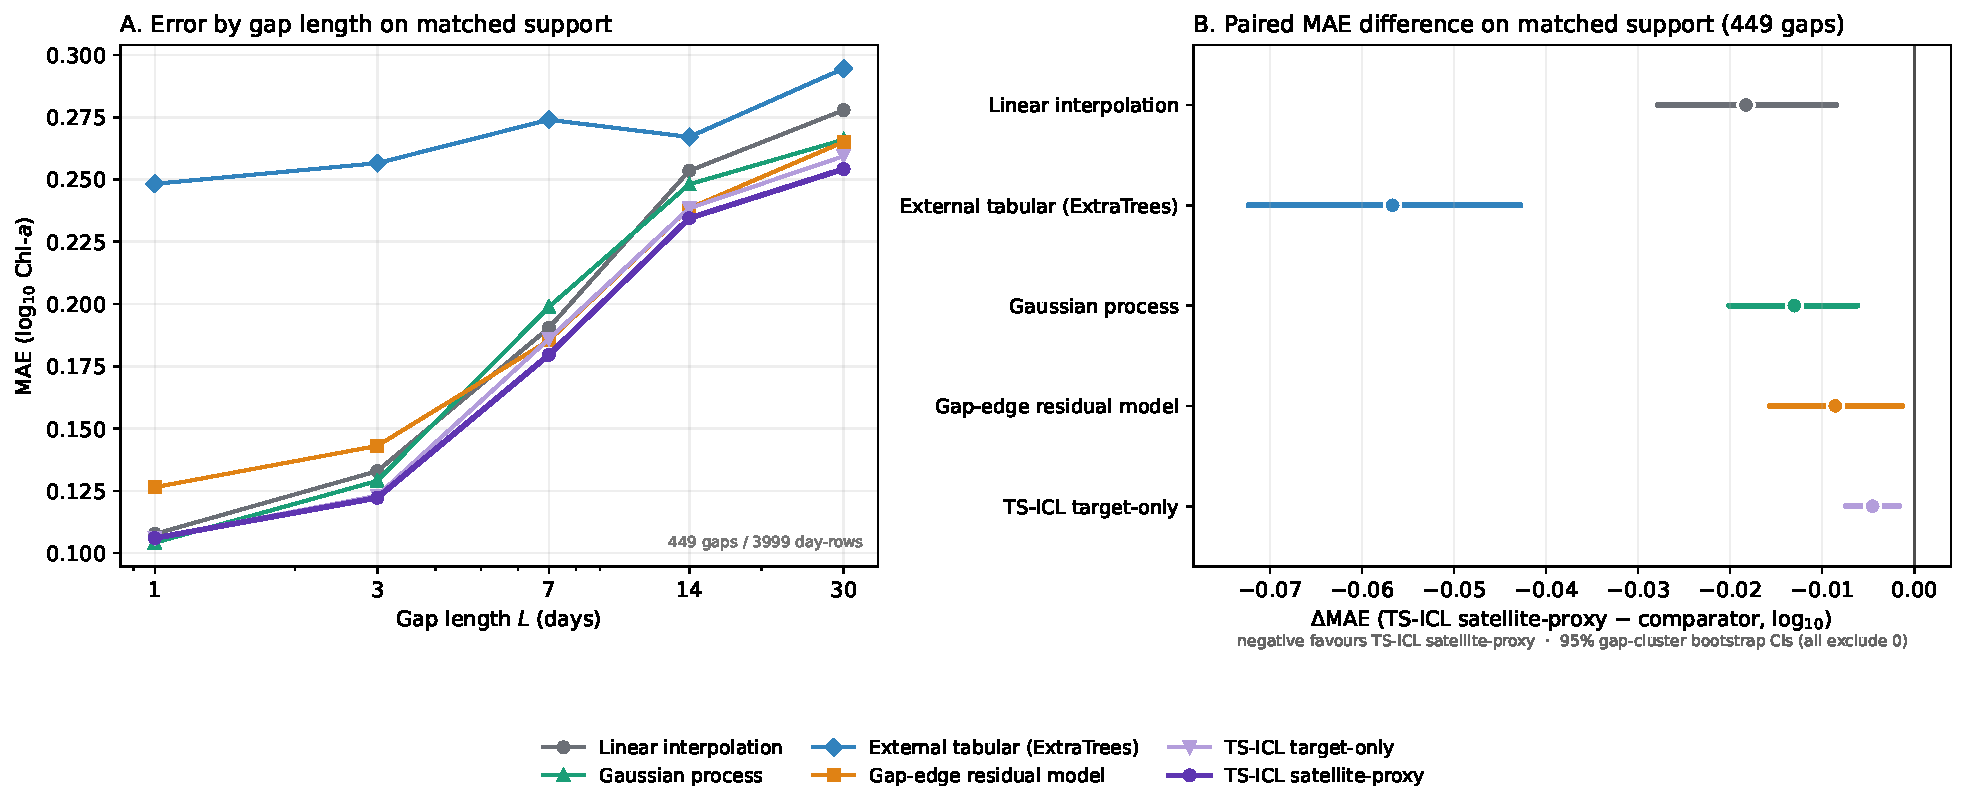
\includegraphics[width=\textwidth]{figures/fig4_chlorophyll_benchmark_matched.pdf}
  \caption{Artificial-gap chlorophyll benchmark.
  (A) Mean absolute error in $\log_{10}$ chlorophyll-\textit{a} by gap length. (B) Paired MAE difference
  between TS-ICL satellite-proxy and each comparator.}
  \label{fig:chl_benchmark_matched}
\end{figure}

TS-ICL also returns quantile predictions, here summarized by q05--q95 intervals. For the satellite-proxy
arm, empirical coverage is close to nominal at the three tested interval widths (Table~\ref{tab:tsicl_calibration}). This indicates that the reported uncertainty bands are generally informative, which matters here because real imputation scenarios have no withheld truth and should not be presented as point estimates alone.

\begin{table}[h]
  \centering
  \caption{TS-ICL satellite-proxy quantile calibration on the full 681-gap diagnostic pool.}
  \label{tab:tsicl_calibration}
  \begin{tabular}{rrr}
    \toprule
    Nominal interval & Empirical coverage & Difference \\
    \midrule
    50\% & 51.3\% & $+$1.3~pp \\
    80\% & 81.8\% & $+$1.8~pp \\
    90\% & 91.6\% & $+$1.6~pp \\
    \bottomrule
  \end{tabular}
\end{table}

\subsection{Covariate-signal checks}
\label{sec:chl_covariate_probe}

The TS-ICL covariate experiments provide a second way to test whether external predictors carry
usable reconstruction information. Unlike tabular feature importance, these checks do not depend
on a particular hand-engineered feature ranking. Each covariate
family is compared with placebo versions that preserve some marginal structure while breaking
the physically meaningful timing. Therefore a family is treated as carrying useful signal only
when the correctly aligned sequence beats the placebo alternatives with confidence intervals excluding zero.

Figure~\ref{fig:chl_covariate_placebo} shows the four-transform placebo battery for the physical
covariate families. Wind/upwelling forcing is the clearest physical signal: the aligned sequence
beats all four placebo variants. A curated physical-forcing set also survives the battery, but
with a smaller effect. Solar radiation gives mixed evidence, and SST/thermal forcing is not
robust under this criterion. Ocean current/transport covariates beat none of the placebo
variants, so the tested current inputs did not establish a usable chlorophyll reconstruction signal.

\begin{figure}[h]
  \centering
  \makebox[\textwidth][c]{%
    \hspace*{-1cm}%
    \resizebox{\textwidth}{!}{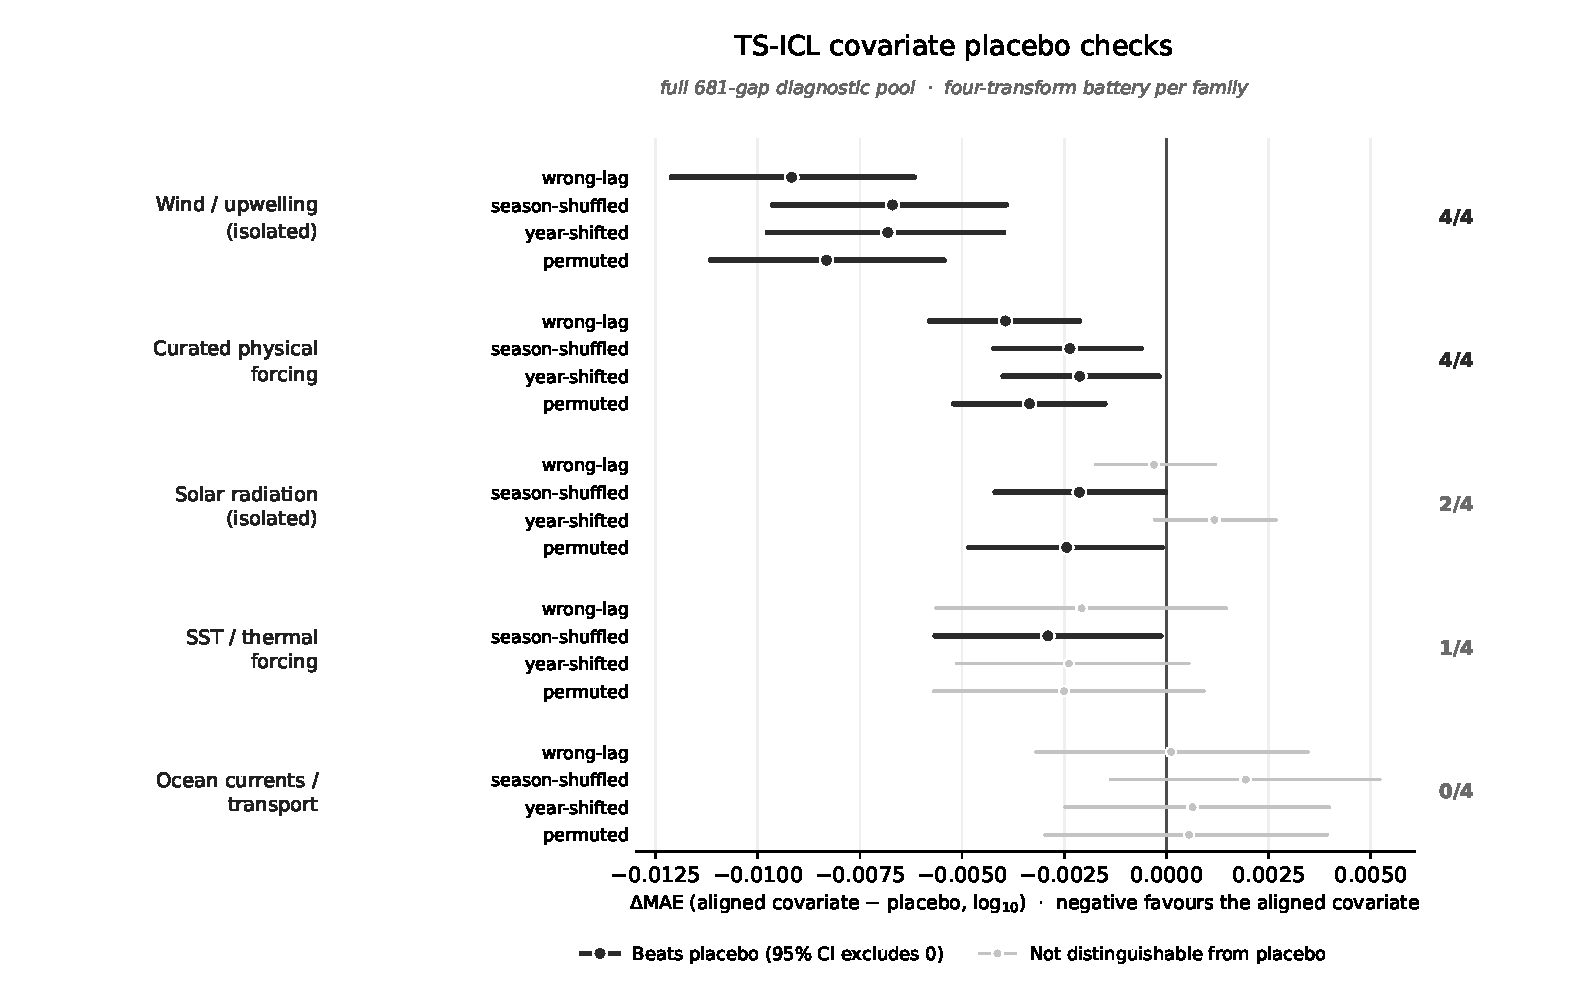
\includegraphics[width=0.92\textwidth]{figures/fig_chl_covariate_placebo_summary_v2.pdf}}%
  }
  \caption{TS-ICL covariate placebo checks for physical predictor families.
  Each row compares the correctly aligned covariate sequence with a disrupted placebo version. This is a full 681-gap TS-ICL diagnostic.}
  \label{fig:chl_covariate_placebo}
\end{figure}

\subsection{High-\texorpdfstring{\chl{}}{Chl-a} events remain difficult}
\label{sec:chl_events}

The benchmark identifies TS-ICL satellite-proxy as the strongest overall method, but the
event-stratified results show a clear limitation. All methods have higher MAE on high-\chl{}
event gaps than on non-event gaps (Figure~\ref{fig:chl_event_limitation}A). The external-only
tabular model is especially weak in this regime, consistent with the broader result that external
predictors alone do not reconstruct the target reliably. The gap-edge residual model and TS-ICL
reduce error relative to the weaker comparators, but neither removes the event penalty.

The illustrative artificial gap in Figure~\ref{fig:chl_event_limitation}B shows the nature of the
failure. The withheld event rises sharply inside the hidden interval. TS-ICL satellite-proxy has
the lowest error among the plotted methods for this gap, but its median reconstruction still
smooths and underestimates the event peak. Bloom events in this region can be short-lived and spatially patchy \citep{chavez2009comparison}, and all methods must infer the hidden event interior from boundary context, external covariates, or both.

\begin{figure}[h]
  \centering
  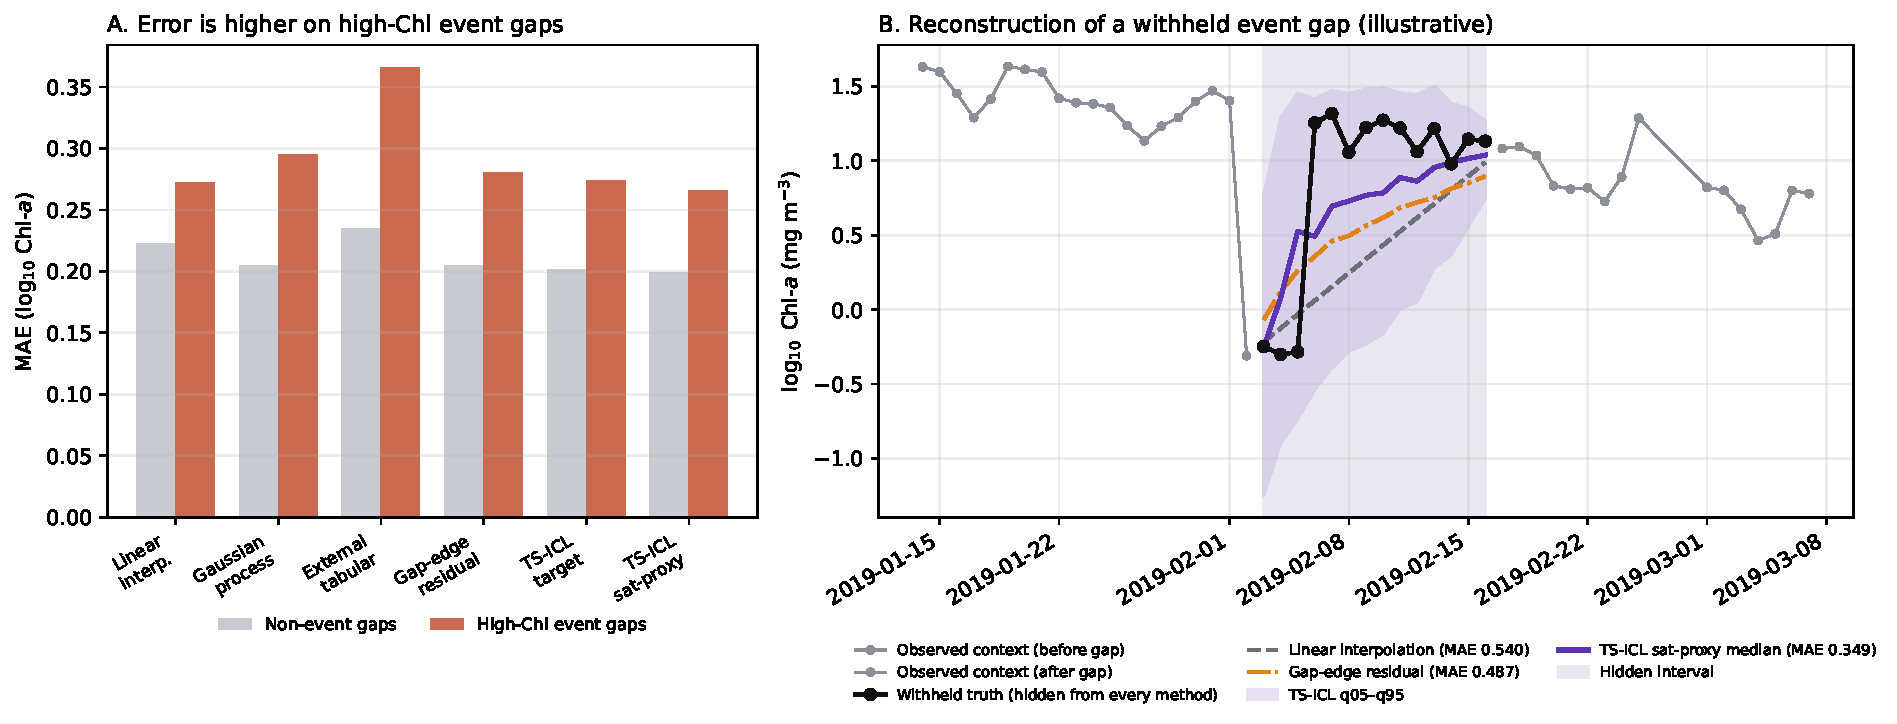
\includegraphics[width=\textwidth]{figures/fig5_event_limitation_matched_v2.pdf}
  \caption{High-\texorpdfstring{\chl{}}{Chl-a} event limitation.
  (A) Event and non-event MAE. All methods have higher error on
  high-\chl{} event gaps. (B) One withheld artificial 14-day event gap, shown as an illustrative
  example. Observed context is shown only outside the
  hidden interval; the black curve is the withheld truth used for artificial-gap scoring. For this
  example, per-gap MAE is 0.540 for linear interpolation, 0.487 for the gap-edge residual model,
  and 0.349 for TS-ICL satellite-proxy, but TS-ICL still underestimates the peak.}
  \label{fig:chl_event_limitation}
\end{figure}

\subsection{Real gaps: illustrative reconstructions, not validation}
\label{sec:chl_realgaps}

The benchmark evaluates reconstruction skill only on artificial gaps, where withheld
truth exists, while on real gaps the target was never observed, so no MAE or method ranking
can be computed. The TS-ICL satellite-proxy method was nevertheless applied to the real
chlorophyll gaps as an illustrative gap-filling output for practical use.

Figure~\ref{fig:chl_real_gap_multigap} shows one continuous 2015--2016 window containing six real
gaps of different lengths: 14, 15, 1, 1, 5, and 45 days.
All six gaps are within the artificial-gap validation range used in this report.
The main point is practical. TS-ICL can produce continuous candidate values across several real interruptions without fitting a separate station-specific model for each gap. The artificial-gap results above indicate how the method behaves when truth is available, while this figure shows how the selected method would be applied to actual missing intervals.

\begin{figure}[h]
  \centering
  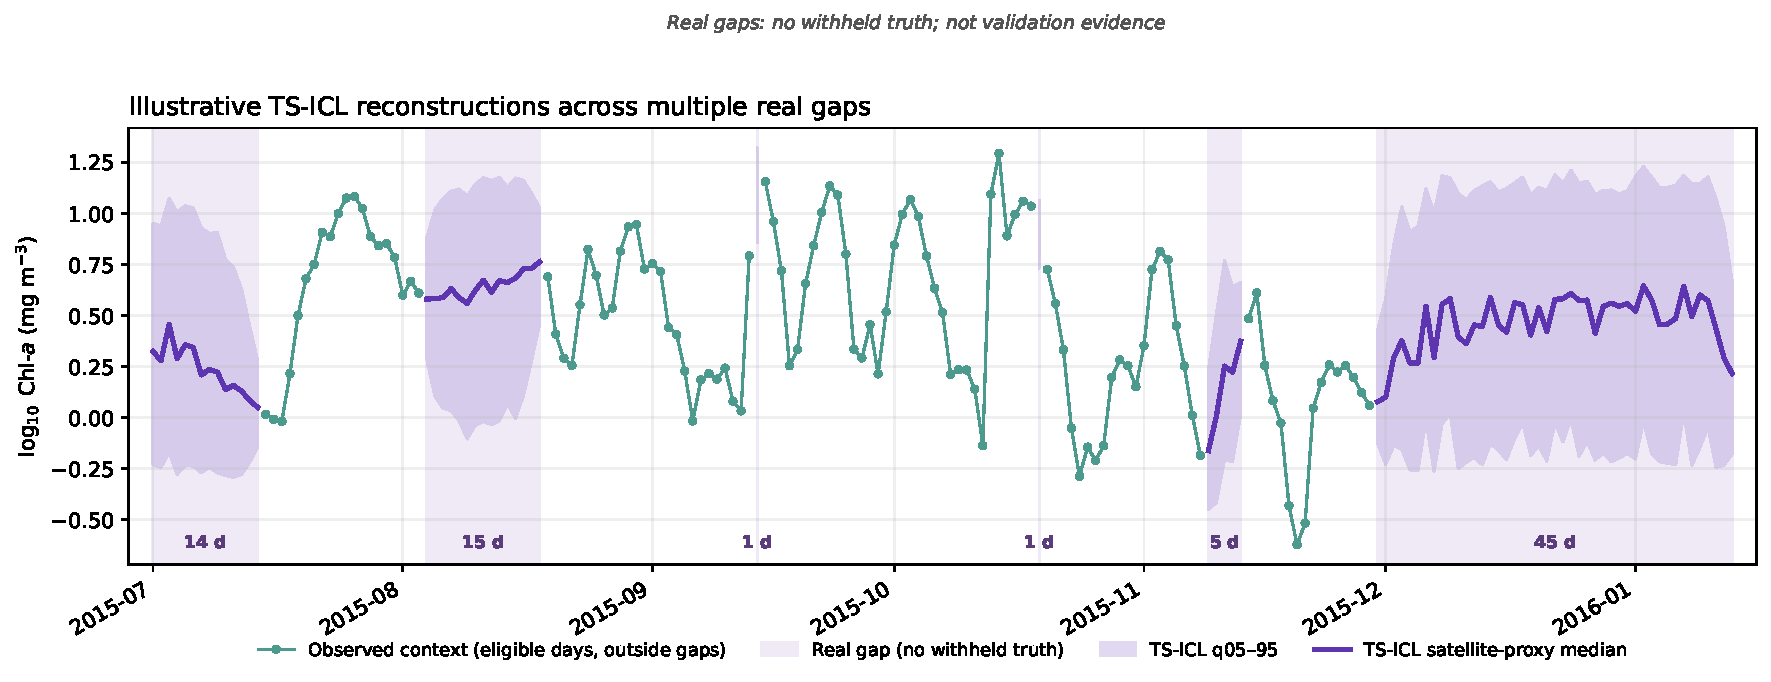
\includegraphics[width=0.95\textwidth]{figures/fig_chl_real_gap_multigap_v1.pdf}
  \caption{Illustrative chlorophyll real-gap reconstructions. A continuous 2015--2016 window is shown with six real gaps.}
  \label{fig:chl_real_gap_multigap}
\end{figure}


\newpage
% ── Section 5: Oxygen case-study results ─────────────────────────────
\section{Oxygen Case Study: A Compact Transfer Benchmark}
\label{sec:oxygen}

Dissolved oxygen provides a second test of the reconstruction workflow developed for
chlorophyll. It is also locally relevant in its own right: oxygen variability in Tongoy Bay is
connected to the environmental conditions affecting scallop aquaculture
\citep{ramajo2019scallops}, and low-oxygen alerts are already used operationally by local
aquaculture actors \citep{ceaza_tongoy_oxygen_alerts_2024}. The purpose of this section is
therefore twofold: to evaluate whether the same benchmark ladder transfers to another sensor, and,
if it does, to identify what changes in the results.

The oxygen benchmark is deliberately more compact than the
chlorophyll case study. We evaluate the same model ladder, but the main claims
are restricted to an artificial-gap range $L=1$--30. This support contains
406 artificial gaps and 2912 hidden target days.

\subsection{Artificial-gap benchmark}
\label{sec:oxygen_benchmark}

Figure~\ref{fig:oxygen_benchmark_primary} summarizes the oxygen benchmark. Linear
interpolation is again the relevant floor: it clearly improves on monthly climatology and
persistence, with a pooled MAE of 0.733~mg/L. The best external-only
tabular configuration has MAE 0.847~mg/L, about 15.5\% worse than interpolation. Thus, as in the
chlorophyll case, external gridded physical predictors alone do not provide a reliable replacement
for local target continuity inside the bay.

The Gaussian process has a MAE of 0.738~mg/L and its
paired confidence interval includes zero, so it is best read as a statistical tie with
interpolation. The gap-edge residual model reaches near-parity at some medium and longer
gap lengths, but it does not provide an overall improvement over interpolation on the considered
range.

The only method that clearly improves on interpolation in the pooled oxygen benchmark is TS-ICL.
The target-only TS-ICL model is better than interpolation at the point-estimate level, but its
paired improvement is not fully resolved. The strongest audited version uses physical covariate
channels, including SST, wind, solar radiation and
current. This version reaches MAE 0.675~mg/L, an 8.0\% reduction relative to
interpolation, with a 95\% gap-cluster bootstrap confidence interval of 4.5--11.4\%.

The broad chlorophyll conclusion therefore transfers only in part: interpolation remains a strong
baseline, external tabular predictors alone do not clear it in the pooled benchmark, and the
zero-shot foundation model gives the strongest pooled reconstruction result. The failure mode,
however, is different and is analysed in Section~\ref{sec:oxygen_tails}. One visible exception in
Figure~\ref{fig:oxygen_benchmark_primary}A is the external-tabular performance at $L=30$; this
stratum contains only 15 gaps, and a robustness audit showed that the apparent reversal is driven
by a small number of high-error interpolation cases, it is therefore treated as diagnostic.

\begin{figure}[h]
  \centering
  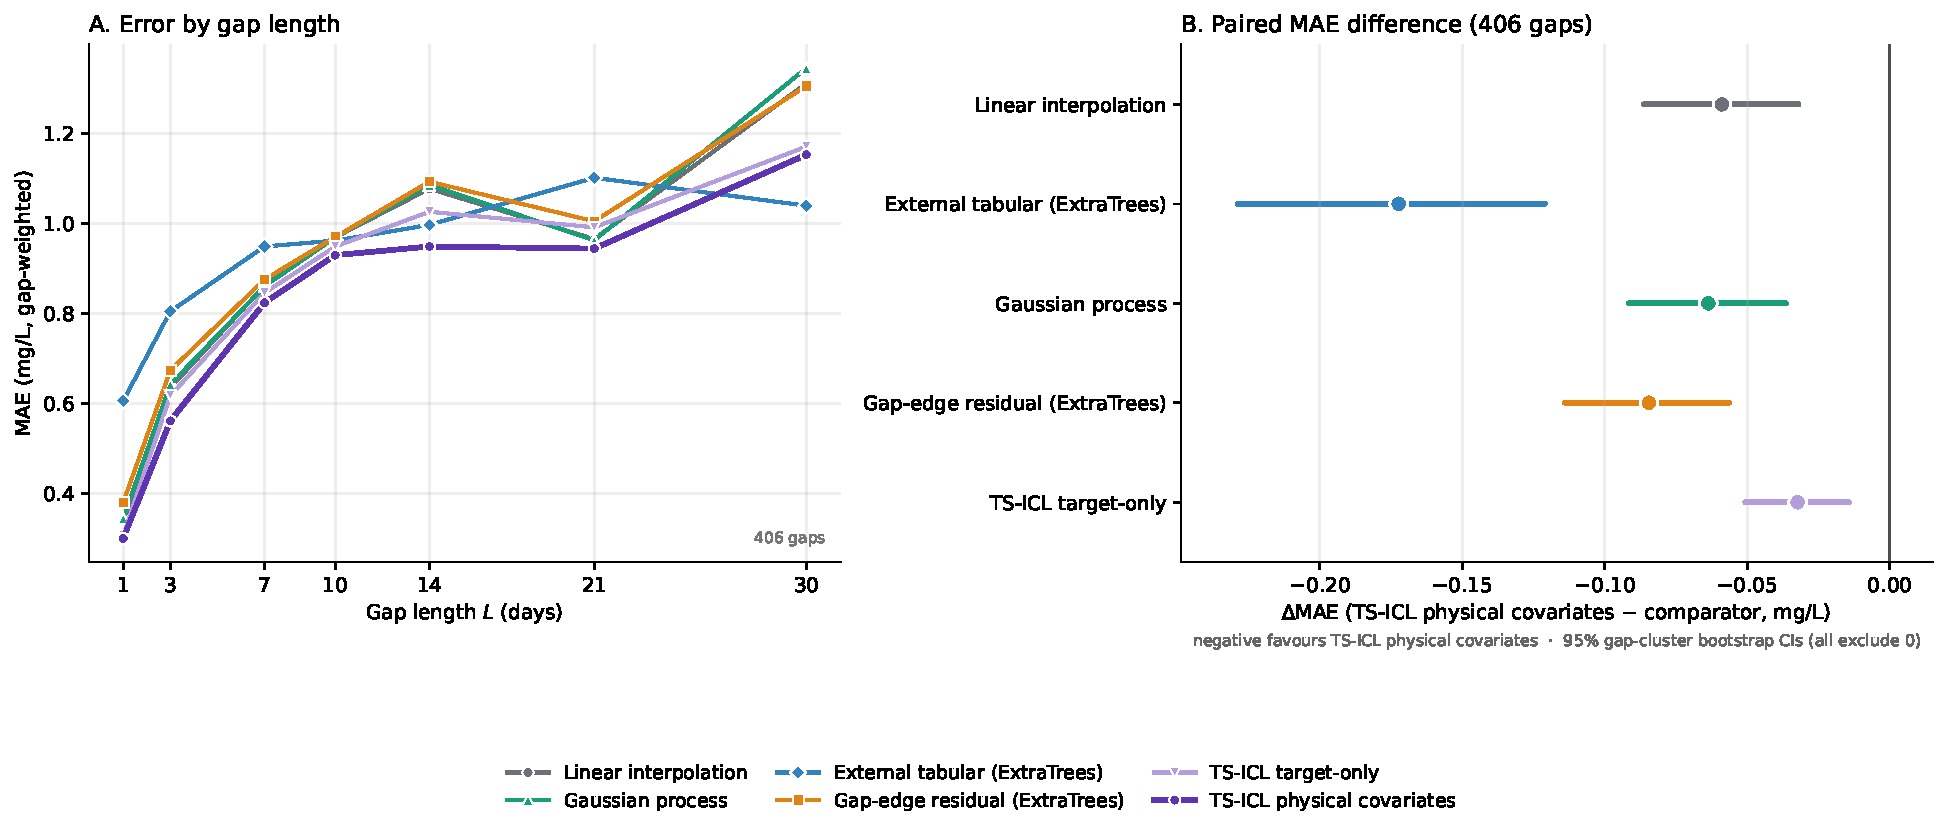
\includegraphics[width=\textwidth]{figures/fig_oxygen_benchmark_primary_v3.pdf}
  \caption{Dissolved-oxygen artificial-gap benchmark.
  (A) Mean absolute error in mg/L by gap length. (B) Pooled paired MAE
  differences between TS-ICL physical covariates and each comparator.}
  \label{fig:oxygen_benchmark_primary}
\end{figure}

\subsection{Physical covariates and distribution-tail limitations}
\label{sec:oxygen_tails}

Running TS-ICL with different covariate arms probes which physical information channels are useful
for oxygen reconstruction. The most informative result concerns current and transport variables:
when added to the broader physical covariate bundle, they do not produce a resolved improvement,
but in isolation the current-only arm is the strongest single-family TS-ICL arm. The
interpretation is that current-derived information is useful, but largely redundant with what the
combined SST, wind and radiation bundle already captures.

TS-ICL's pooled improvement over interpolation is not uniform across the oxygen distribution
(Figure~\ref{fig:oxygen_tail_diagnostics}). The gain is concentrated in the middle of the empirical
oxygen distribution, especially the p10--p25 and p25--p50 bands. At the point-estimate level,
TS-ICL is worse than interpolation in both tails. 

The persistence split sharpens the same point. The largest diagnostic failures occur in sustained
tail runs rather than isolated tail excursions, especially in the sustained high tail. That stratum
is small, so the magnitude should be interpreted cautiously, but the qualitative pattern is
consistent with regression toward the centre of the training distribution: TS-ICL tends to
overpredict low oxygen and underpredict high oxygen.

Two physical associations help interpret the tail pattern but remain exploratory. Same-day solar
radiation is negatively correlated with oxygen ($r=-0.41$), so a simple productivity-driven
high-oxygen explanation is not supported. The low-oxygen tail is enriched in austral spring under
stronger upwelling, while the high-oxygen tail is enriched in summer under weaker upwelling,
suggesting that broad physical forcing contributes to the tail structure.

\begin{figure}[h]
  \centering
  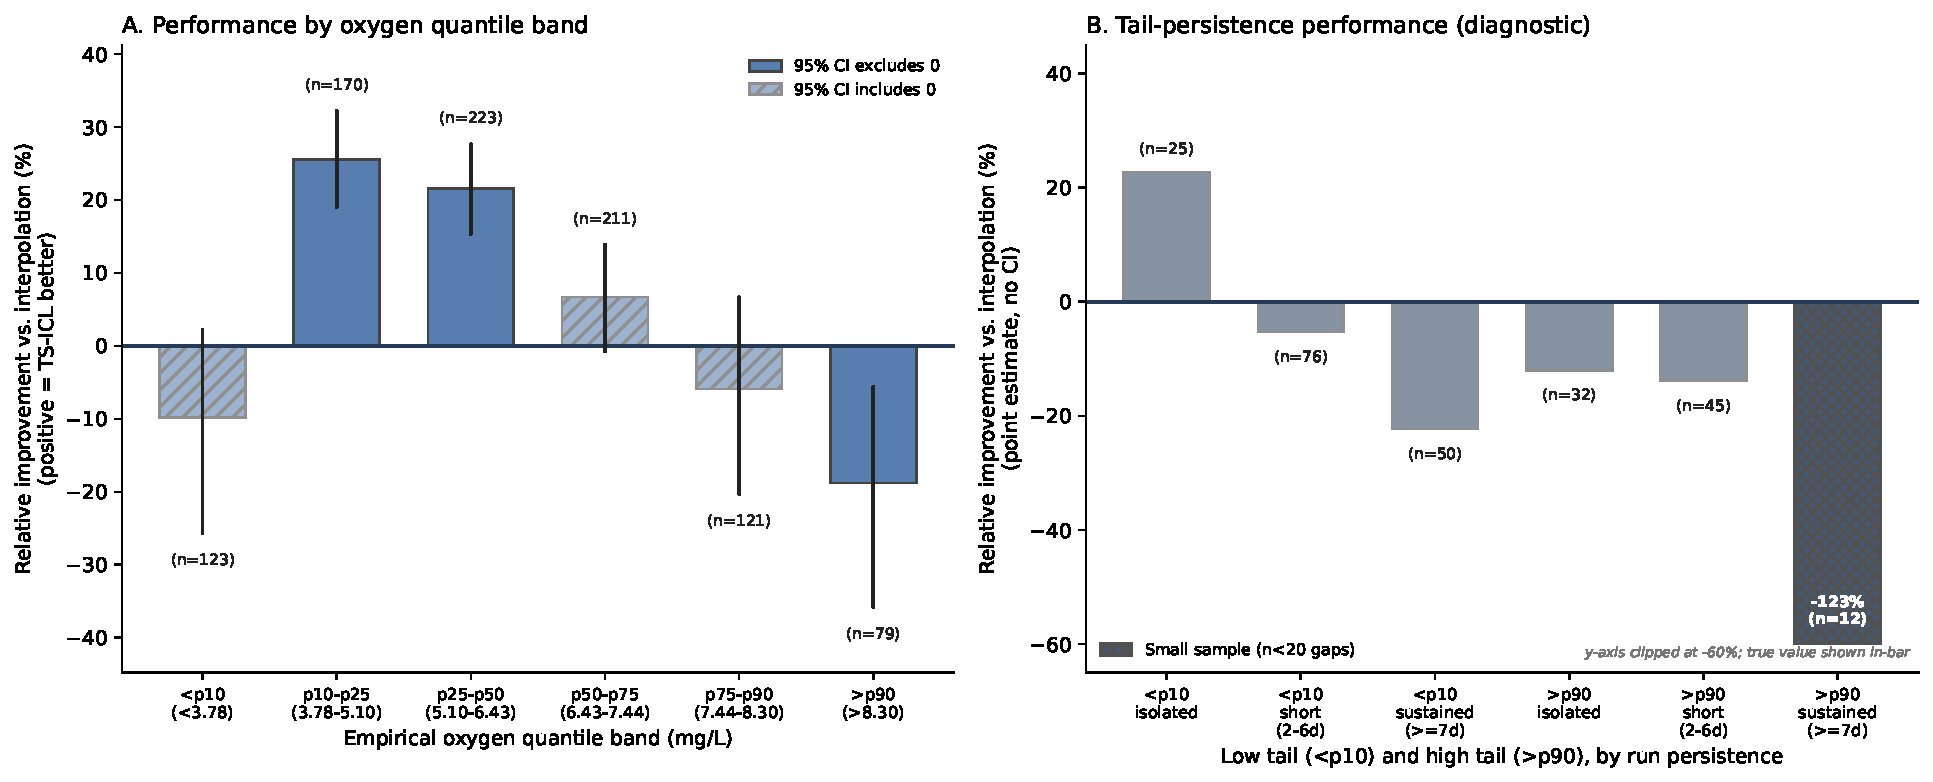
\includegraphics[width=\textwidth]{figures/fig_oxygen_tail_diagnostics_v6.pdf}
  \caption{Dissolved-oxygen distribution-tail diagnostics.
  (A) Relative improvement of the strongest TS-ICL arm over interpolation across empirical
  oxygen quantile bands. (B) Tail-persistence diagnostic for low-oxygen and high-oxygen tail runs. Quantile bands are empirical validation strata, not ecological
  thresholds.}
  \label{fig:oxygen_tail_diagnostics}
\end{figure}

\newpage
% ── Section 6: Cross-case synthesis ─────────────────────────────
\section{Cross-Case Synthesis}
\label{sec:synthesis}

Chlorophyll and
dissolved oxygen respond to overlapping but different physical and biological processes, have
different distributions, and fail in different regimes. The transferable object is therefore the
benchmark workflow itself: define a daily target, construct artificial gaps, enforce leakage control and
compare methods against withheld truth. Under that workflow, the two targets show a consistent methodological
hierarchy but different scientific failure modes.

\subsection{What transfers across targets}
\label{sec:synthesis_transfers}

The first transferable result is that interpolation is a strong floor. In both case studies, simple
target continuity explains a large fraction of the recoverable signal, especially at short gaps. Methods that add
external predictors or model complexity must therefore be judged asking whether they improve on the information already carried by the local target trajectory.

The second transferable result is that external tabular prediction alone is not enough. For both
chlorophyll and oxygen, the external-only model is worse than interpolation. This means that, when
used as day-wise external predictors without target context, physical forcing data do not reliably replace the
local continuity of the in-situ record. In a nearshore bay, gridded products can carry useful physical
information while still being too coarse to reconstruct the sensor target by themselves.

The third transferable result is that pretrained sequence modelling adds skill beyond this floor.
TS-ICL is the strongest chlorophyll method on both benchmarks and this is operationally important because the model is used
zero-shot, which means its parameters are not fitted or fine-tuned on Tongoy data. 

\subsection{What changes between targets}
\label{sec:synthesis_changes}

The covariate evidence is target-specific. For chlorophyll, the clearest physical signal is
wind forcing, while the tested current inputs do not establish a useful
reconstruction signal. This is consistent with a biological target whose short events are linked to
upwelling and surface biomass but are also spatially patchy and difficult for coarse external products
to capture. For oxygen, current information behaves differently: it is informative in
isolation, but largely redundant when added to the broader physical covariate bundle. The same
predictor family can therefore matter differently depending on the target and on the other covariates
already present.

The main failure mode also changes. For chlorophyll, the hardest regime is high-\chl{} events, since every method has higher error on event gaps than on non-event gaps. For oxygen, the TS-ICL improvement
is concentrated in the middle of the empirical distribution, while the tails remain difficult. The same general lesson is that the method
that wins on average is not automatically reliable in the regimes that matter most scientifically.

This distinction is important for interpretation and therefore the benchmark needs both
pooled comparison and stratified diagnostics. Without the latter, the chlorophyll result
would overstate event skill and the oxygen one would have done the same with tail reliability.

\subsection{Implications for operational reconstruction}
\label{sec:synthesis_operational}

The practical implication of the results is the following. First, any candidate method should be benchmarked against
linear interpolation under artificial gaps. Second, external predictors should be tested as empirical
information channels and not assumed useful from physical plausibility alone. Third, a selected
reconstruction method should be accompanied by regime diagnostics.

This is where TS-ICL is operationally attractive. Once the target and covariate channels are
prepared, it does not require fitting a station-specific model for each sensor or rebuilding a
large engineered tabular design. Inference is fast, and the same framework can ingest target
history and covariates as time-indexed channels rather than forcing temporal awareness into a
large set of hand-built lags, rolling summaries, and gap-edge columns. The channel structure also
makes diagnostic tests straightforward: a covariate family can be added, removed, or replaced by
placebo versions to test whether it carries time-aligned information. Eventually, the reconstruction is not only a point estimate but a candidate trajectory
with an uncertainty band, which is a key factor in real gaps scenarios.
\newpage
% ── Section 7: Limitations and future work ─────────────────────────────
\section{Limitations and Future Work}
\label{sec:limitations_future}

The previous section identified the main transferable pattern: interpolation is a strong floor,
external predictors alone are not sufficient, TS-ICL adds skill, and the hardest regimes are
the distributional extremes. This final section states where those conclusions stop and what should be tested next.
The main deliverable that this reported framework gives CEAZA
is a reproducible way to decide when a reconstruction is credible, when it is only useful as a candidate
trajectory, and where new physical features or models are needed.

\subsection{Validation support and gap-length limits}
\label{sec:limits_validation}

The benchmark validates reconstruction skill only where artificial gaps can be created from
observed eligible data. This is a strong design choice, because every scored reconstruction is
compared with withheld truth, but it also limitats the validation support useful for the imputation of real gaps.

Real gaps sit in fact outside this validation logic. The real-gap reconstructions, shown for example in
Figure~\ref{fig:chl_real_gap_multigap}, are useful practical outputs for future research activities that benefit from continuous records, but they are not evidence of
method skill because the target was not observed inside those intervals. This distinction is
especially important for long outages: the shared 256-day station-wide gap during the 2020 pandemic, and other very long
real gaps, are longer than the artificial gaps used for model ranking. Any reconstruction of
such intervals is extrapolation from the validated regime, not a validated result.

\subsection{Extremes remain the main unresolved regime}
\label{sec:limits_extremes}

The most important limitation is not the ranking on a limited artificial-gap support, but the behaviour of the methods in the regimes that matter most scientifically. For chlorophyll, this means high-\chl{} event gaps, where Figure~\ref{fig:chl_event_limitation} shows that every method has higher error: even the best method still smooths sharp blooms and underestimates event peaks.
For oxygen, the corresponding limitation is again on the empirical tails of the distribution. TS-ICL improves in the benchmark because it performs better in the middle of
the oxygen distribution, but Figure~\ref{fig:oxygen_tail_diagnostics} shows weaker behaviour in the low and high tails, especially when tail conditions persist. The oxygen result therefore gives a
clear example of why a pooled MAE improvement is not enough for full operational trust: the average can
improve while the scientifically sensitive strata remain unreliable. Future work should therefore make event and tail performance part of the objective, not only a
post-hoc diagnostic. For chlorophyll, this could mean event-aware validation and modelling, with
losses or selection criteria that explicitly penalize missed bloom peaks. For oxygen, it means
separating isolated tail excursions from sustained tail episodes and testing whether models can
avoid regression toward the centre of the distribution. 

\subsection{Physical interpretation and covariate limits}
\label{sec:limits_physical}

The covariate analyses are a useful product to identify reconstructive signal from physical forcing predictors. For chlorophyll, it's wind/upwelling forcing that establishes useful signal, while for oxygen it's current information that proves being more informative, although it appears redundant once combined with
the broader physical covariate bundle. These findings do not
prove that the corresponding physical processes are causal, but are anyway useful because they
show which information channels improve reconstruction and indicates this approach as a future pipeline/research tool.

This distinction between causality and reconstruction improvement matters in Tongoy Bay because the relevant processes occur across scales. The
available gridded products describe regional surface chlorophyll, SST, winds and currents, but the
in-situ sensors measure conditions at a nearshore buoy inside a bay. Short-lived blooms, retention,
local circulation and aquaculture-scale variability may be only indirectly represented in the external products. A
negative reconstruction result for a predictor family therefore cannot be read as ruling out the
underlying process.

A natural extension is to design physical features more directly around the unresolved regimes. For
chlorophyll, this means testing whether wind history, local retention, recent cooling or
spatial patchiness can better anticipate bloom formation and decay. For oxygen, it means building
features that distinguish sustained low- or high-oxygen episodes from isolated excursions, and
testing whether current variables contribute unique information once the broader physical
state is controlled.

\subsection{Model and uncertainty limits}
\label{sec:limits_models_uncertainty}

TS-ICL is promising here because it improves in the benchmark for both targets without station-specific fitting or fine-tuning, and because it can use target history and covariates as
time-indexed channels rather than relying on a large hand-built tabular feature matrix. But this
does not make it a universal solution, as only one pretrained time-series imputation foundation model was tested,
and the results do not establish that TS-ICL is the best architecture available for coastal
imputation, tabular foundation models being a first natural extension. Anyway, in this scenarios where datasets have a limited size and covariates on coarse grids may not explain well nearshore measurements, the results establish that this class of zero-shot models deserves comparison against classical baselines.

The uncertainty evidence is also incomplete. For chlorophyll for instance, TS-ICL satellite-proxy quantile
intervals are close to nominal overall, but event-day calibration is weaker. Future work should treat interval calibration as a first-class benchmark output.

A further model-level limitation is boundary behaviour. Boundary-anchored methods such as linear
interpolation and gap-edge residual models are constrained by observations at the edges of an
internal gap. TS-ICL uses a broader context window and covariate channels, and is not explicitly
forced to match the nearest observations at the gap boundary. This can be an advantage when local
endpoints are misleading, but it can also create edge discontinuities. A practical next step is to
test hybrid methods that preserve TS-ICL's interior reconstruction while blending more conservatively near the gap edges.

\subsection{Extensions of the benchmark workflow}
\label{sec:future_extensions}

The main reusable output of this report is the benchmark workflow. A new sensor or station can be
processed through the same sequence: define the daily target and eligibility rule, audit missingness,
construct artificial gaps, apply leakage-controlled comparators, stratify errors by scientifically
relevant regimes, and only then produce real-gap reconstructions if the evidence supports them.

Several extensions follow directly from this structure. The first is spatial transfer: applying the
same benchmark to other CEAZA stations would test whether the model hierarchy found at Tongoy is
specific to this site or network-wide. The second is target transfer: additional variables such as
temperature, salinity, turbidity, pH or other biogeochemical sensors could be evaluated with the
same design. The third is long-gap validation: longer artificial gaps are rare because they require
long uninterrupted observed runs, so pooling multiple stations or alternative validation designs
may be needed to evaluate outages beyond the current support.
\newpage

% ── References ─────────────────────────────────────────────
\bibliographystyle{apalike}
\bibliography{references}
\newpage

% ── Appendix  ─────────────────────────────────────────────
\appendix
% ── Appendix: Technical reproducibility and extended diagnostics ─────────────
\section{Technical Reproducibility and Extended Diagnostics}
\label{sec:appendix_repro}

This appendix records the technical details needed to interpret and reproduce the report's main
results. The accompanying GitHub repository \citep{faverio2026coastal_gap_repository} contains the
complete scripts, feature matrices, per-gap prediction tables, model outputs, and extended diagnostic
files. The appendix instead reports the target definitions, validation supports, product provenance,
benchmark backing tables, and selected robustness diagnostics needed to make the main text auditable.

\subsection{Target definitions and daily quality control}
\label{app:targets_qc}

Both targets are daily means computed from hourly Tongoy buoy (BTG) observations from the CEAZAMET
BTG station \citep{ceazamet_btg_station}. A day is eligible only if at least 18 hourly observations
are valid. Chlorophyll is modelled and scored on $\log_{10}(\texttt{chl\_mean})$, while dissolved
oxygen is modelled and scored directly in mg/L.

\begin{table}[h]
  \centering
  \small
  \caption{Daily target definitions and quality-control summaries. The date span for both targets
  is 2015-07-01 to 2026-05-31, for a total of 3988 possible daily records.}
  \label{tab:appendix_target_qc}
  \begin{tabularx}{\textwidth}{@{}l l l r r r r@{}}
    \toprule
    Target & Channel & Unit & Eligible days & Missing days & Missing share & Real gaps \\
    \midrule
    Chlorophyll-a
    & BTGCLF
    & mg~m$^{-3}$
    & 3012
    & 976
    & 24.5\%
    & 128 \\

    Dissolved oxygen
    & BTGOXD2
    & mg/L
    & 2880
    & 1108
    & 27.8\%
    & 125 \\
    \bottomrule
  \end{tabularx}
\end{table}

\begin{table}[h]
  \centering
  \small
  \caption{Distribution summaries for eligible daily target values.}
  \label{tab:appendix_target_distributions}
  \begin{tabular}{l r r r r}
    \toprule
    Target & Median & IQR & p05 & p95 \\
    \midrule
    Chlorophyll-a (mg~m$^{-3}$)
    & 3.48 & 5.04 & 0.79 & 15.93 \\

    Dissolved oxygen (mg/L)
    & 6.43 & 2.34 & 2.82 & 8.80 \\
    \bottomrule
  \end{tabular}
\end{table}

\subsection{External products and provenance}
\label{app:data_products}

External products are used as predictor channels. Table~\ref{tab:appendix_products}
extends the compact product summary in the main text.

\begin{table}[h]
  \centering
  \small
  \caption{External products used to construct report predictor channels.}
  \label{tab:appendix_products}
  \begin{tabularx}{\textwidth}{@{}l X l l X@{}}
    \toprule
    Product / source & Role in report & Native scale & Coverage & Notes \\
    \midrule
    CEAZAMET BTG / PLV
    & In-situ sensor targets and local atmospheric forcing.
    & point, hourly
    & --
    & BTG provides the chlorophyll and oxygen targets; PLV provides local meteorological forcing. \\

    GlobColour L4 \chl{}
    & Satellite biological proxy for surface chlorophyll.
    & $\sim$4~km, daily
    & $\sim$90\%
    & \\

    MUR SST
    & Sea-surface temperature and thermal-state predictors.
    & $\sim$1~km, daily
    & $\sim$98\%
    & Used for SST and thermal forcing summaries. \\

    CMEMS winds
    & Regional wind and upwelling forcing predictors.
    & $\sim$25~km, hourly
    & $\sim$90\%
    & Used for wind speed, stress and upwelling-related summaries. \\

    GLORYS12 currents
    & Regional current and transport predictors.
    & $\sim$8~km, daily
    & $>99\%$
    & Used for current speed, components and transport summaries. \\
    \bottomrule
  \end{tabularx}
\end{table}

\subsection{Artificial-gap pools and validation supports}
\label{app:gap_pools}

\begin{table}[h]
  \centering
  \small
  \caption{Artificial-gap pools and report validation supports.}
  \label{tab:appendix_gap_supports}
  \begin{tabularx}{\textwidth}{@{}l l l r X@{}}
    \toprule
    Target & Support & Gap lengths & Gaps & Role in report \\
    \midrule
    Chlorophyll
    & Full TS-ICL pool
    & $1,3,7,10,14,21,30,45,60$
    & 681
    & TS-ICL calibration and covariate-signal diagnostics. \\

    Chlorophyll
    & Shared ladder support
    & $1,3,7,14,30$
    & 449
    & Main chlorophyll method ranking; all headline comparators evaluated on the same hidden intervals. \\

    Oxygen
    & Primary support
    & $1,3,7,10,14,21,30$
    & 406
    & Main oxygen method ranking and distribution-tail diagnostics. \\

    Oxygen
    & Exploratory longer support
    & $>30$
    & 6
    & Not used for headline oxygen claims. \\
    \bottomrule
  \end{tabularx}
\end{table}
\vspace{-0.5cm}
\subsection{Feature construction}
\label{app:feature_model_details}

The main text groups predictors into scientific information channels: calendar/seasonality, target
history, satellite biological proxy, wind/upwelling forcing, SST, and
current/transport information. Tabular models require these channels to be converted into explicit
per-day feature vectors. TS-ICL accepts time-indexed covariate channels, which may still be engineered summaries, but they enter as channels over time rather than as one fixed row of
tabular features per hidden day.

\begin{small}
\setlength{\tabcolsep}{4pt}
\renewcommand{\arraystretch}{1.18}

\begin{longtable}{P{2.4cm}P{3.2cm}P{4.9cm}P{4.4cm}P{1cm}}  \caption{Feature-construction inventory.}
  \label{tab:appendix_feature_construction} \\
  \toprule
  Feature family & Raw source & Constructed features & Physical meaning & Target \\
  \midrule
  \endfirsthead

  \toprule
  Feature family & Raw source & Constructed features & Physical meaning & Target \\
  \midrule
  \endhead

  \bottomrule
  \endfoot

  Calendar / seasonality
  & Timestamp
  & \begin{tabitemize}[leftmargin=*, nosep, topsep=0pt]
    \item month
    \item year
    \item sine/cosine doy
  \end{tabitemize}
  & Position within the annual upwelling and productivity cycle.
  & Both \\

  Target history
& Target record before the gap.
& \begin{tabitemize}[leftmargin=*, nosep, topsep=0pt]
    \item 3-, 7-, and 14-day pre-gap statistics;
    \item short pre-gap slopes;
  \end{tabitemize}
& Trend of the observed target approaching the missing interval.
& Both \\

  Gap-edge context
  & Target record on both gap sides
  & \begin{tabitemize}[leftmargin=*, nosep, topsep=0pt]
    \item first pre/post-gap values;
    \item gap-position geometry;
    \item edge-to-edge mean, slope;
  \end{tabitemize}
  & Behaviour bracketing an internal gap, used to correct interpolation.
  & Both \\

  Satellite biological proxy
  & GlobColour L4 \chl{} \citep{garnesson2019globcolour}.
  & \begin{tabitemize}[leftmargin=*, nosep, topsep=0pt]
    \item nearest-cell log-\chl{};
    \item $3\times3$ / $5\times5$ box summaries;
    \item patchiness, gradients;
    \item doy/moy anomalies;
  \end{tabitemize}
  & Regional surface chlorophyll as an external proxy for the in-situ biological signal.
  & CLF \\

  Wind / upwelling forcing
  & PLV station winds and CMEMS winds \citep{copernicus_wind_l4}
  & \begin{tabitemize}[leftmargin=*, nosep, topsep=0pt]
    \item wind components/speed;
    \item upwelling indices;
    \item wind-direction persistence;
    \end{tabitemize}
  & Mechanical forcing of coastal upwelling.
  & Both \\

  Solar / atmospheric forcing
  & PLV meteorology.
  & \begin{tabitemize}[leftmargin=*, nosep, topsep=0pt]
    \item radiation lags and rolling means;
    \item pressure/humidity summaries;
  \end{tabitemize}
  & Local radiative and atmospheric state over the bay.
  & Both \\

  SST / thermal state
  & MUR SST \citep{jpl_mur_sst}
  & \begin{tabitemize}[leftmargin=*, nosep, topsep=0pt]
    \item nearest-cell SST;
    \item cooling indices;
    \item coastal gradients;
  \end{tabitemize}
  & Thermal tracer of recently upwelled water and surface stratification.
  & Both \\

  Current / transport
  & GLORYS12 currents \citep{lellouche2021glorys12,copernicus_glorys12}
  & \begin{tabitemize}[leftmargin=*, nosep, topsep=0pt]
    \item current speed/components;
    \item alongshore and cross-shore;
    \item divergence, vorticity, Okubo Weiss;
  \end{tabitemize}
  & Advection, exchange, and retention conditions over the shelf.
  & Both \\

  Local BTG diagnostics
  & BTG water temperature and pressure.
  & \begin{tabitemize}[leftmargin=*, nosep, topsep=0pt]
    \item daily mean;
    \item valid hour count;
  \end{tabitemize}
  & Co-located physical state at the buoy, distinct from the oxygen sensor.
  & OXY \\
\end{longtable}
\end{small}

\subsection{Chlorophyll benchmark backing tables}
\label{app:chl_benchmark_tables}

This subsection gives the numerical backing for the matched chlorophyll benchmark in
Section~\ref{sec:chl_benchmark}. All values are computed on $\log_{10}(\texttt{chl\_mean})$.

\begin{table}[h]
  \centering
  \small
  \caption{Chlorophyll benchmark summary.}
  \label{tab:appendix_chl_matched_metrics}
  \begin{tabular}{l r}
    \toprule
    Method & MAE \\
    \midrule
    TS-ICL satellite-proxy & 0.221 \\
    TS-ICL target-only & 0.225 \\
    Gap-edge residual & 0.229 \\
    Gaussian process & 0.234 \\
    Linear interpolation & 0.239 \\
    External tabular (ExtraTrees) & 0.277 \\
    External tabular (HGB) & 0.287 \\
    \bottomrule
  \end{tabular}
\end{table}

\begin{table}[h]
  \centering
  \small
  \caption{Chlorophyll MAE by gap length.}
  \label{tab:appendix_chl_by_length}
  \begin{tabular}{r r r r r r r}
    \toprule
    $L$ & Linear interp. & Gaussian process & External tabular & Gap-edge & TS target & TS satellite \\
    \midrule
    1  & 0.108 & 0.104 & 0.248 & 0.127 & 0.106 & 0.106 \\
    3  & 0.133 & 0.129 & 0.257 & 0.143 & 0.123 & 0.122 \\
    7  & 0.190 & 0.199 & 0.274 & 0.185 & 0.186 & 0.180 \\
    14 & 0.254 & 0.248 & 0.267 & 0.239 & 0.239 & 0.235 \\
    30 & 0.278 & 0.266 & 0.295 & 0.265 & 0.259 & 0.254 \\
    \bottomrule
  \end{tabular}
\end{table}

\begin{table}[H]
  \centering
  \small
  \caption{Paired chlorophyll MAE differences against TS-ICL satellite-proxy.}
  \label{tab:appendix_chl_paired_deltas}
  \begin{tabular}{l r r}
    \toprule
    Comparator & $\Delta$MAE & 95\% CI \\
    \midrule
    Linear interpolation & -0.018 & [-0.028,\,-0.008] \\
    External tabular (ExtraTrees) & -0.057 & [-0.072,\,-0.043] \\
    Gaussian process & -0.013 & [-0.020,\,-0.006] \\
    Gap-edge residual & -0.009 & [-0.016,\,-0.001] \\
    TS-ICL target-only & -0.005 & [-0.007,\,-0.002] \\
    \bottomrule
  \end{tabular}
\end{table}

\subsection{Chlorophyll event diagnostics}
\label{app:chl_extended_diagnostics}

High-\chl{} events remain difficult for all methods. Table~\ref{tab:appendix_chl_event_mae}
reports the event/non-event split used to support Figure~\ref{fig:chl_event_limitation}.

\begin{table}[H]
  \centering
  \small
  \caption{Chlorophyll event and non-event MAE.}
  \label{tab:appendix_chl_event_mae}
  \begin{tabular}{l r r}
    \toprule
    Method & Non-event MAE & High-\chl{} event MAE \\
    \midrule
    Linear interpolation & 0.223 & 0.272 \\
    Gaussian process & 0.204 & 0.295 \\
    External tabular (ExtraTrees) & 0.235 & 0.366 \\
    Gap-edge residual & 0.205 & 0.281 \\
    TS-ICL target-only & 0.202 & 0.274 \\
    TS-ICL satellite-proxy & 0.199 & 0.266 \\
    \bottomrule
  \end{tabular}
\end{table}

\subsection{Oxygen benchmark backing tables}
\label{app:oxygen_benchmark_tables}

This subsection gives the numerical backing for the primary oxygen benchmark in
Section~\ref{sec:oxygen_benchmark}. All oxygen MAE values are gap-weighted and reported in mg/L.

\begin{table}[H]
  \centering
  \small
  \caption{Oxygen benchmark by gap length.}
  \label{tab:appendix_oxygen_by_length}
  \begin{tabular}{r r r r r r r r}
    \toprule
    $L$ & $n$ & Interp. & Ext. tabular & GP & Gap-edge & TS target & TS physical \\
    \midrule
    1  & 100 & 0.339 & 0.606 & 0.345 & 0.380 & 0.307 & 0.300 \\
    3  & 100 & 0.635 & 0.805 & 0.642 & 0.674 & 0.618 & 0.562 \\
    7  & 78  & 0.863 & 0.949 & 0.861 & 0.876 & 0.846 & 0.824 \\
    10 & 55  & 0.970 & 0.962 & 0.970 & 0.971 & 0.949 & 0.930 \\
    14 & 36  & 1.078 & 0.998 & 1.086 & 1.094 & 1.027 & 0.949 \\
    21 & 22  & 0.966 & 1.102 & 0.963 & 1.005 & 0.992 & 0.945 \\
    30 & 15  & 1.312 & 1.040 & 1.346 & 1.306 & 1.171 & 1.153 \\
    \bottomrule
  \end{tabular}
\end{table}

\begin{table}[h]
  \centering
  \small
  \caption{Paired oxygen MAE differences against TS-ICL physical covariates.}
  \label{tab:appendix_oxygen_paired_deltas}
  \begin{tabular}{l r r}
    \toprule
    Comparator & $\Delta$MAE (mg/L) & 95\% CI \\
    \midrule
    Linear interpolation & -0.059 & [-0.086,\,-0.032] \\
    External tabular (ExtraTrees) & -0.172 & [-0.229,\,-0.121] \\
    Gaussian process & -0.064 & [-0.091,\,-0.036] \\
    Gap-edge residual (ExtraTrees) & -0.084 & [-0.114,\,-0.056] \\
    TS-ICL target-only & -0.032 & [-0.051,\,-0.014] \\
    \bottomrule
  \end{tabular}
\end{table}

The external-tabular curve appears favourable at $L=30$ in the by-length plot, but this stratum has
only 15 gaps. A focused robustness audit was therefore used to decide whether this local reversal
should be treated as a headline result. Table~\ref{tab:appendix_oxygen_l30_audit} shows why it is
kept as a diagnostic caveat only.

\begin{table}[h]
  \centering
  \small
  \caption{Oxygen $L=30$ external-tabular robustness audit.}
  \label{tab:appendix_oxygen_l30_audit}
  \begin{tabularx}{\textwidth}{@{}l X@{}}
    \toprule
    Diagnostic & Result \\
    \midrule
    Number of $L=30$ gaps
    & 15 \\

    Bootstrap 95\% CI for mean paired difference
    & [-0.644,\,+0.092] mg/L; includes zero. \\

    Most influential gap
    & \texttt{OX\_L030\_20241115}, where interpolation has very high error. \\

    Sensitivity interpretation
    & The apparent mean reversal is influenced by a small number of high-error interpolation
      cases. \\

    Median / trimmed comparison
    & Alternative summaries still show some external-tabular advantage, but the mean advantage is
      not confidence-interval resolved. \\

    Report interpretation
    & Small-stratum diagnostic, not a headline reversal of the pooled conclusion. \\
    \bottomrule
  \end{tabularx}
\end{table}

\subsection{Oxygen tail diagnostics}
\label{app:oxygen_extended_diagnostics}

The oxygen distribution-tail diagnostics use empirical quantile bands, not ecological thresholds.
Relative improvement is computed against interpolation.
The high-tail loss in Table~\ref{tab:appendix_oxygen_quantile_bands} is confidence-interval
resolved, while the low-tail loss is a point-estimate loss whose confidence interval includes zero.
The tail-persistence split sharpens the diagnostic pattern but uses smaller strata, especially for
sustained high oxygen, and is therefore not treated as a separate headline comparison.

\begin{table}[h]
  \centering
  \small
  \caption{Oxygen TS-ICL performance by empirical oxygen quantile band.}
  \label{tab:appendix_oxygen_quantile_bands}
  \begin{tabular}{l r r r}
    \toprule
    Band & $n$ & Relative improvement & 95\% CI \\
    \midrule
    $<p10$ ($<3.78$ mg/L) & 123 & -9.8\% & [-25.7,\,+2.2]\% \\
    $p10$--$p25$ (3.78--5.10 mg/L) & 170 & +25.5\% & [+19.0,\,+32.2]\% \\
    $p25$--$p50$ (5.10--6.43 mg/L) & 223 & +21.6\% & [+15.3,\,+27.6]\% \\
    $p50$--$p75$ (6.43--7.44 mg/L) & 211 & +6.7\% & [-0.8,\,+13.9]\% \\
    $p75$--$p90$ (7.44--8.30 mg/L) & 121 & -5.9\% & [-20.3,\,+6.7]\% \\
    $>p90$ ($>8.30$ mg/L) & 79 & -18.8\% & [-35.8,\,-5.6]\% \\
    \bottomrule
  \end{tabular}
\end{table}

\begin{table}[H]
  \centering
  \small
  \caption{Oxygen tail-persistence diagnostics.}
  \label{tab:appendix_oxygen_tail_persistence}
  \begin{tabular}{l r r}
    \toprule
    Tail-persistence stratum & $n$ & Relative improvement vs interpolation \\
    \midrule
    Low tail, isolated & 25 & 23.1\% \\
    Low tail, short run (2--6 d) & 76 & -5.2\% \\
    Low tail, sustained run ($\geq$7 d) & 50 & -22.3\% \\
    High tail, isolated & 32 & -12.3\% \\
    High tail, short run (2--6 d) & 45 & -13.8\% \\
    High tail, sustained run ($\geq$7 d) & 12 & -123.4\% \\
    \bottomrule
  \end{tabular}
\end{table}

\end{document}
